\documentclass[11pt,a4paper]{report}

% -----------------------------------------------------------------------------
% PACKAGES & SYSTEM CONFIGURATION
% -----------------------------------------------------------------------------
\usepackage[utf8]{inputenc}
\usepackage[T1]{fontenc}
\usepackage[a4paper, top=2.5cm, bottom=2.5cm, left=2.5cm, right=2.5cm]{geometry}
\usepackage{amsmath, amssymb, amsthm}
\usepackage{graphicx}
\usepackage{booktabs, multirow, tabularx}
\usepackage{tikz, pgfplots}
\usepackage{algorithm}
\usepackage{algpseudocode}
\usepackage{subcaption}
\usepackage{listings}
\usepackage{xcolor}
\usepackage{microtype}
\usepackage{url}
\usepackage[numbers,sort&compress]{natbib}
\usepackage[hidelinks,colorlinks=true,linkcolor=blue!70!black,citecolor=teal!70!black,urlcolor=blue!70!black]{hyperref}
\usepackage{cleveref}

% TikZ libraries
\usetikzlibrary{shapes.geometric, arrows.meta, positioning, calc, fit, backgrounds, patterns}
\pgfplotsset{compat=1.18}

% Theorem Environments
\newtheorem{theorem}{Theorem}[chapter]
\newtheorem{proposition}[theorem]{Proposition}
\newtheorem{lemma}[theorem]{Lemma}
\newtheorem{corollary}[theorem]{Corollary}
\theoremstyle{definition}
\newtheorem{definition}[theorem]{Definition}
\newtheorem{example}[theorem]{Example}
\theoremstyle{remark}
\newtheorem{remark}[theorem]{Remark}

% Listings styling
\definecolor{codegreen}{rgb}{0,0.6,0}
\definecolor{codegray}{rgb}{0.5,0.5,0.5}
\definecolor{codepurple}{rgb}{0.58,0,0.82}
\definecolor{backcolour}{rgb}{0.96,0.97,0.98}

\lstdefinestyle{mystyle}{
    backgroundcolor=\color{backcolour},   
    commentstyle=\color{codegreen},
    keywordstyle=\color{magenta},
    numberstyle=\tiny\color{codegray},
    stringstyle=\color{codepurple},
    basicstyle=\ttfamily\footnotesize,
    breakatwhitespace=false,         
    breaklines=true,                 
    captionpos=b,                    
    keepspaces=true,                 
    numbers=left,                    
    numbersep=5pt,                  
    showspaces=false,                
    showstringspaces=false,
    showtabs=false,                  
    tabsize=2
}
\lstset{style=mystyle}

% -----------------------------------------------------------------------------
% TITLE & METADATA
% -----------------------------------------------------------------------------
\title{
    \vspace{-2cm}
    \textbf{\Large NATIONAL POLYTECHNIC UNIVERSITY OF ARMENIA}\\
    \textbf{\large Institute of Information and Telecommunication Technologies and Electronics}\\
    \textbf{\normalsize Department of Software Engineering and Computer Systems}\\[1.5cm]
    \rule{\linewidth}{1.2pt}\\[0.4cm]
    {\huge \textbf{Game World Modeling Using Machine Learning Methods}}\\[0.2cm]
    {\LARGE \textbf{GLDtk: A Neuro-Symbolic, Mixed-Initiative Pipeline for Statically Verified 2D Platformer Level Generation in LDtk}}\\[0.4cm]
    \rule{\linewidth}{1.2pt}\\[0.6cm]
    {\normalsize \textbf{Armenian Title:} Խաղային աշխարհների մոդելավորում մեքենայական ուսուցման մեթոդներով}\\[1cm]
    \textbf{Master's Thesis Dissertation}
}

\author{
    \textbf{Candidate:} Bekiryan\\
    \textbf{Academic Advisor:} Faculty of Software Engineering\\
    \textbf{Target Editor:} LDtk 1.5.3 (Level Designer Toolkit)
}

\date{November 2026}

\begin{document}

\maketitle

% -----------------------------------------------------------------------------
% ABSTRACT & KEYWORDS
% -----------------------------------------------------------------------------
\begin{abstract}
Designing 2D platformer game worlds is a labor-intensive engineering discipline requiring simultaneous mastery of continuous Newtonian kinematics, discrete progression topology, spatial clearance constraints, and cohesive visual composition. Existing generative level design methodologies face a fundamental \textbf{Procedural Content Generation (PCG) Trilemma}: (1)~\emph{Classical constructive and constraint-based algorithms} (e.g., WaveFunctionCollapse, Tanagra, Dormans mission grammars) enforce local tile consistency or topological validity but lack open-ended natural language expressiveness; (2)~\emph{Pure Machine Learning and Large Language Model (LLM) generators} (e.g., MarioGPT, Word2World) provide high semantic controllability from unstructured prompts but suffer from severe \emph{spatial blindness}---frequently synthesizing impassable jump chasms, low-ceiling hitbox collisions, unreachable progression items, and irreversible soft-locks; and (3)~\emph{Academic mixed-initiative prototypes} (e.g., Sentient Sketchbook, Morai Maker) remain confined to isolated, non-commercial research sandboxes isolated from professional level editors.

This dissertation presents \textbf{GLDtk} (\emph{Generative Level Design Toolkit}), a neuro-symbolic, mixed-initiative level generation pipeline integrated natively inside Sébastien Bénard's \textbf{LDtk 1.5.3} level editor via a compiled Haxe/Electron sidebar panel. GLDtk decouples \textbf{creative semantic intent} (orchestrated by schema-constrained cloud and local LLMs, augmented with a Retrieval-Augmented Generation pattern index and cross-project Design Memory) from \textbf{geometric realization and formal verification} (governed by deterministic procedural rock carvers, a closed-form kinematic Physics Oracle, and graph-theoretic state-space model checking). Every generated level and local edit is statically verified: swept $12 \times 24\text{ px}$ AABB hitbox trajectories prove reachability across parabolic jumps ($\frac{1}{2}gt^2 - vt + \Delta y = 0$), chained double-jumps with an $\mathcal{O}(1)$ analytical launch optimum $\tau^*$, air dashes, depth-bounded wall-jump climbs, and piecewise cross-section gravity fields. Furthermore, GLDtk guarantees global \textbf{soft-lock freedom}---proving that from \emph{every} reachable platform and inventory state, an Exit remains reachable---using Tarjan Strongly Connected Components (SCC) condensation and a bounded Inventory-State Product Automaton ($\mathcal{S} = V_{\text{standable}} \times \mathcal{P}(\text{Items})$).

Empirical evaluations across a 35-prompt benchmark suite demonstrate that GLDtk achieves \textbf{100\% verified playability}, \textbf{0\% exported soft-locks}, and \textbf{0.95--1.00 prompt fidelity} on frontier models. For local open-weight 14B models (\texttt{qwen2.5:14b}), deterministic symbolic patching alone boosts verification success from \textbf{0\% (0/6) to 83.3\% (5/6)} on identical recorded outputs. The RAG pattern stamping engine achieves \textbf{100\% (4/4)} verified coverage across all structural terrain types at section heights of 20--40 tiles. In side-by-side human-AI authoring trials, GLDtk accelerates end-to-end multi-section level construction by \textbf{4.89$\times$} compared to manual authoring in LDtk (\textbf{1m 13s vs. 5m 57s}).
\end{abstract}

\vspace{0.5cm}
\noindent \textbf{Keywords:} Procedural Content Generation, Neuro-Symbolic AI, Large Language Models, Mixed-Initiative Game Design, LDtk, Kinematic Verification, Soft-Lock Freedom, Tarjan SCC, Mission Grammars, Retrieval-Augmented Generation.

\tableofcontents
\listoffigures
\listoftables

% -----------------------------------------------------------------------------
% CHAPTER 1: INTRODUCTION & PROJECT MOTIVATION
% -----------------------------------------------------------------------------
\chapter{Introduction: Origin, Motivation, and the PCG Trilemma}
\label{chap:intro}

\section{Motivation and Thesis Assignment}
Level design in modern 2D platforming games is an intricate, multi-layered discipline. Unlike open-world 3D sandboxes where navigation can often tolerate approximate geometry, a 2D platformer level acts as a strict spatial program governed by continuous Newtonian physics and discrete state machines. When a game designer positions two stone ledges over a pit of hazards, they must intuitively or analytically simulate five interdependent kinematic and spatial variables:
\begin{enumerate}
    \item The player's horizontal run speed ($v_x$).
    \item The initial vertical jump impulse ($v_y$).
    \item Gravitational acceleration ($g$) and its directional scaling across level sections.
    \item Hitbox envelope dimensions ($w \times h$) relative to surrounding ceiling overhangs.
    \item Active player ability states (such as double jumps, horizontal air dashes, and wall kicks).
\end{enumerate}

Failure to align any of these variables results in broken geometry: an impossible jump, an inescapable pit, or a soft-lock where a player expends a key on the wrong door and becomes permanently stranded.

In academic and commercial practice, automated level authoring has emerged as a promising solution to reduce production bottlenecks. However, existing techniques remain fragmented. As formulated in the official National Polytechnic University of Armenia (NPUA) thesis assignment, the core scientific inquiry of this research is:

\begin{quote}
\textbf{Central Research Question:} \emph{Can we synthesize the unconstrained natural-language creativity of Large Language Models (System 1) with deterministic symbolic physics verification, graph grammars, and procedural geometry engines (System 2) inside an industry-standard level editor (LDtk), such that a designer can describe or iteratively sculpt a 2D game world in plain text and receive a level that is mathematically proven to be beatable, soft-lock free, and faithful to their design intent?}
\end{quote}

\section{The Procedural Content Generation (PCG) Trilemma}
\label{sec:trilemma}

To formalize the architectural motivation behind GLDtk, we define \textbf{The PCG Trilemma} (\Cref{fig:trilemma}). In procedural and generative level design, an autonomous or semi-autonomous system rarely satisfies all three vertices simultaneously without architectural compromise:

\begin{figure}[htbp]
\centering
\begin{tikzpicture}[scale=1.1, every node/.style={align=center}]
    % Triangle coordinates
    \coordinate (A) at (0, 4.2);
    \coordinate (B) at (-4.5, -1.0);
    \coordinate (C) at (4.5, -1.0);
    
    % Draw triangle edges
    \draw[thick, color=slate!60!black, line width=1.5pt] (A) -- (B) -- (C) -- cycle;
    
    % Shaded center
    \fill[color=blue!5, rounded corners=12pt] (-2.2,0.2) rectangle (2.2,2.4);
    
    % Center Node: GLDtk
    \node at (0, 1.3) [draw=blue!80!black, fill=blue!10, rounded corners=6pt, line width=1.4pt, inner sep=8pt] {
        \textbf{\large GLDtk}\\[2pt]
        \footnotesize \textbf{Neuro-Symbolic LDtk Pipeline}\\
        \scriptsize System 1 (LLM) $+$ System 2 (Kinematics) $+$ LDtk
    };
    
    % Vertex A: Expressiveness
    \node at (A) [above=6pt, draw=purple!80!black, fill=purple!10, rounded corners=5pt, inner sep=6pt] {
        \textbf{Vertex A: Creative Expressiveness}\\
        \footnotesize Open-Ended Semantics \& Natural Language Prompting\\
        \scriptsize \emph{Dominant: Pure LLMs (MarioGPT, Word2World)}\\
        \scriptsize \textcolor{red!80!black}{\textbf{Failure:}} Spatial Blindness \& Coordinate Hallucination
    };
    
    % Vertex B: Guarantees
    \node at (B) [below=6pt, draw=green!60!black, fill=green!10, rounded corners=5pt, inner sep=6pt] {
        \textbf{Vertex B: Mathematical Guarantees}\\
        \footnotesize Formal Solvability \& Soft-Lock Freedom\\
        \scriptsize \emph{Dominant: Solvers \& Grammars (Tanagra, Sturgeon)}\\
        \scriptsize \textcolor{red!80!black}{\textbf{Failure:}} Combinatorial Explosion \& Semantic Rigidity
    };
    
    % Vertex C: Production Tooling
    \node at (C) [below=6pt, draw=orange!80!black, fill=orange!10, rounded corners=5pt, inner sep=6pt] {
        \textbf{Vertex C: Production Tooling}\\
        \footnotesize Industrial Studio Integration \& Mixed-Initiative\\
        \scriptsize \emph{Dominant: Native Editors (LDtk, Tiled)}\\
        \scriptsize \textcolor{red!80!black}{\textbf{Failure:}} Manual Labor Overhead \& Lack of Autonomy
    };
    
    % Edge labels
    \node at (-2.8, 1.9) [rotate=48, font=\scriptsize, color=gray!90!black] {Lacks Solvability Proofs};
    \node at (2.8, 1.9) [rotate=-48, font=\scriptsize, color=gray!90!black] {Lacks Semantic Control};
    \node at (0, -1.4) [font=\scriptsize, color=gray!90!black] {Lacks Industrial Editor Integration};
\end{tikzpicture}
\caption{The Procedural Content Generation (PCG) Trilemma in 2D platformer level design, showing GLDtk's neuro-symbolic placement at the intersection of creative expressiveness, mathematical solvability, and production tool integration.}
\label{fig:trilemma}
\end{figure}

\begin{enumerate}
    \item \textbf{Vertex A: Creative Expressiveness (Unconstrained Natural Language Semantics):}
    Systems powered by generative machine learning (such as MarioGPT~\citep{sudhakaran2023mariogpt} and Word2World~\citep{nasir2024word2world}) accept colloquial user prompts and generate high-level thematic narratives. However, because autoregressive Transformers sample token sequences without spatial ground truth, they suffer from \emph{spatial blindness}---producing impossible jumps, misaligned tile grids, and soft-locks.
    
    \item \textbf{Vertex B: Mathematical Playability Guarantees (Formal Verification \& Solvability):}
    Constructive solvers, Answer Set Programming (ASP), Boolean Satisfiability (SAT), and graph grammar pipelines (e.g., Tanagra~\citep{smith2011tanagra}, Launchpad~\citep{smith2011launchpad}, Sturgeon~\citep{cooper2022sturgeon}, and Dormans mission grammars~\citep{dormans2010adventures, dormans2011generating}) provide mathematical guarantees of solvability. However, they lack natural language understanding; modifying level aesthetics or high-level pacing requires re-authoring intricate formal constraint systems or rule bases. Furthermore, solver complexity scales exponentially ($O(2^n)$ in the worst case) with canvas dimensions.
    
    \item \textbf{Vertex C: Production Tooling \& Mixed-Initiative Integration:}
    Commercial game development relies on dedicated, hardware-accelerated 2D level editors such as Sébastien Bénard's Level Designer Toolkit (LDtk)~\citep{benard2020ldtk} or Tiled. While these editors provide rich visual tools, autotiling brushes, and JSON export pipelines, they are fundamentally passive: every tile, obstacle, and entity must be placed manually. Conversely, academic PCG prototypes almost universally deliver throwaway custom user interfaces~\citep{liapis2013sentient, guzdial2019morai} that cannot be integrated into a studio's version-controlled game project.
\end{enumerate}

GLDtk resolves this trilemma by implementing a \textbf{Kahneman Dual-Process Architecture}~\citep{kahneman2011thinking, garcez2023neurosymbolic}:
\begin{itemize}
    \item \textbf{System 1 (Intuitive, Generative, Heuristic):} A fine-tuned or prompt-orchestrated Large Language Model (Gemini, Claude, or local Qwen) parses developer prompts, reasons about thematic pacing, selects spatial archetypes, and emits a structured specification schema (\texttt{LevelSpec}).
    \item \textbf{System 2 (Deliberative, Logical, Deductive):} A deterministic symbolic engine evaluates the proposal against continuous kinematic equations ($\frac{1}{2}gt^2 - vt + \Delta y = 0$), extracts rasterized tile spans, verifies swept hitboxes, enforces Tarjan SCC soft-lock freedom, and patches geometric defects algorithmically without invoking redundant LLM inferences.
    \item \textbf{Mixed-Initiative Substrate:} The resulting level is loaded natively into LDtk 1.5.3 via an embedded Electron/Haxe sidebar, supporting seam-locked regional regeneration, live Route Overlays, interactive 60~Hz playtesting, and continuous Design Memory learning.
\end{itemize}

\section{The Four-Generation Evolution of the Architecture (v1 to v4)}
The GLDtk architecture evolved across four major iterations during development:

\begin{figure}[htbp]
\centering
\begin{tikzpicture}[node distance=1.0cm and 0.8cm, auto,
    block/.style={rectangle, draw=blue!70!black, fill=blue!5, rounded corners=4pt, text width=3.3cm, minimum height=2.2cm, font=\scriptsize, align=center},
    arrow/.style={-{Stealth[scale=1.1]}, thick, color=slate!80!black}]
    
    \node [block] (v1) {\textbf{\normalsize Generation 1 (v1)}\\[3pt]
    \textbf{Topological Sugiyama}\\[2pt]
    $\bullet$ Abstract node/edge graph\\
    $\bullet$ 4-phase Sugiyama layout\\
    $\bullet$ Basic 1-jump Oracle\\
    $\bullet$ Floating platforms in void};
    
    \node [block, right=of v1] (v2) {\textbf{\normalsize Generation 2 (v2)}\\[3pt]
    \textbf{Grounded Neuro-Symbolic}\\[2pt]
    $\bullet$ Pydantic \texttt{LevelSpec} schema\\
    $\bullet$ Grid swept-hitbox re-verify\\
    $\bullet$ Multi-ability \texttt{GameProfile}\\
    $\bullet$ Native Haxe LDtk sidebar};
    
    \node [block, right=of v2] (v3) {\textbf{\normalsize Generation 3 (v3)}\\[3pt]
    \textbf{Procedural Rock Carving}\\[2pt]
    $\bullet$ 7 rock structure carvers\\
    $\bullet$ Boundary port alignment\\
    $\bullet$ Comfort-first jump limits\\
    $\bullet$ In-editor 60\,Hz Play Mode};
    
    \node [block, right=of v3] (v4) {\textbf{\normalsize Generation 4 (v4)}\\[3pt]
    \textbf{Metroidvania \& RAG}\\[2pt]
    $\bullet$ Tarjan SCC soft-lock proof\\
    $\bullet$ Item-State Automaton\\
    $\bullet$ Dormans Mission Grammars\\
    $\bullet$ RAG Pattern Stamping};
    
    \draw [arrow] (v1) -- (v2);
    \draw [arrow] (v2) -- (v3);
    \draw [arrow] (v3) -- (v4);
\end{tikzpicture}
\caption{Four-generation architectural evolution of GLDtk from a topological DAG prototype to a full Metroidvania RAG production pipeline.}
\label{fig:four_gen}
\end{figure}

\begin{figure}[htbp]
\centering
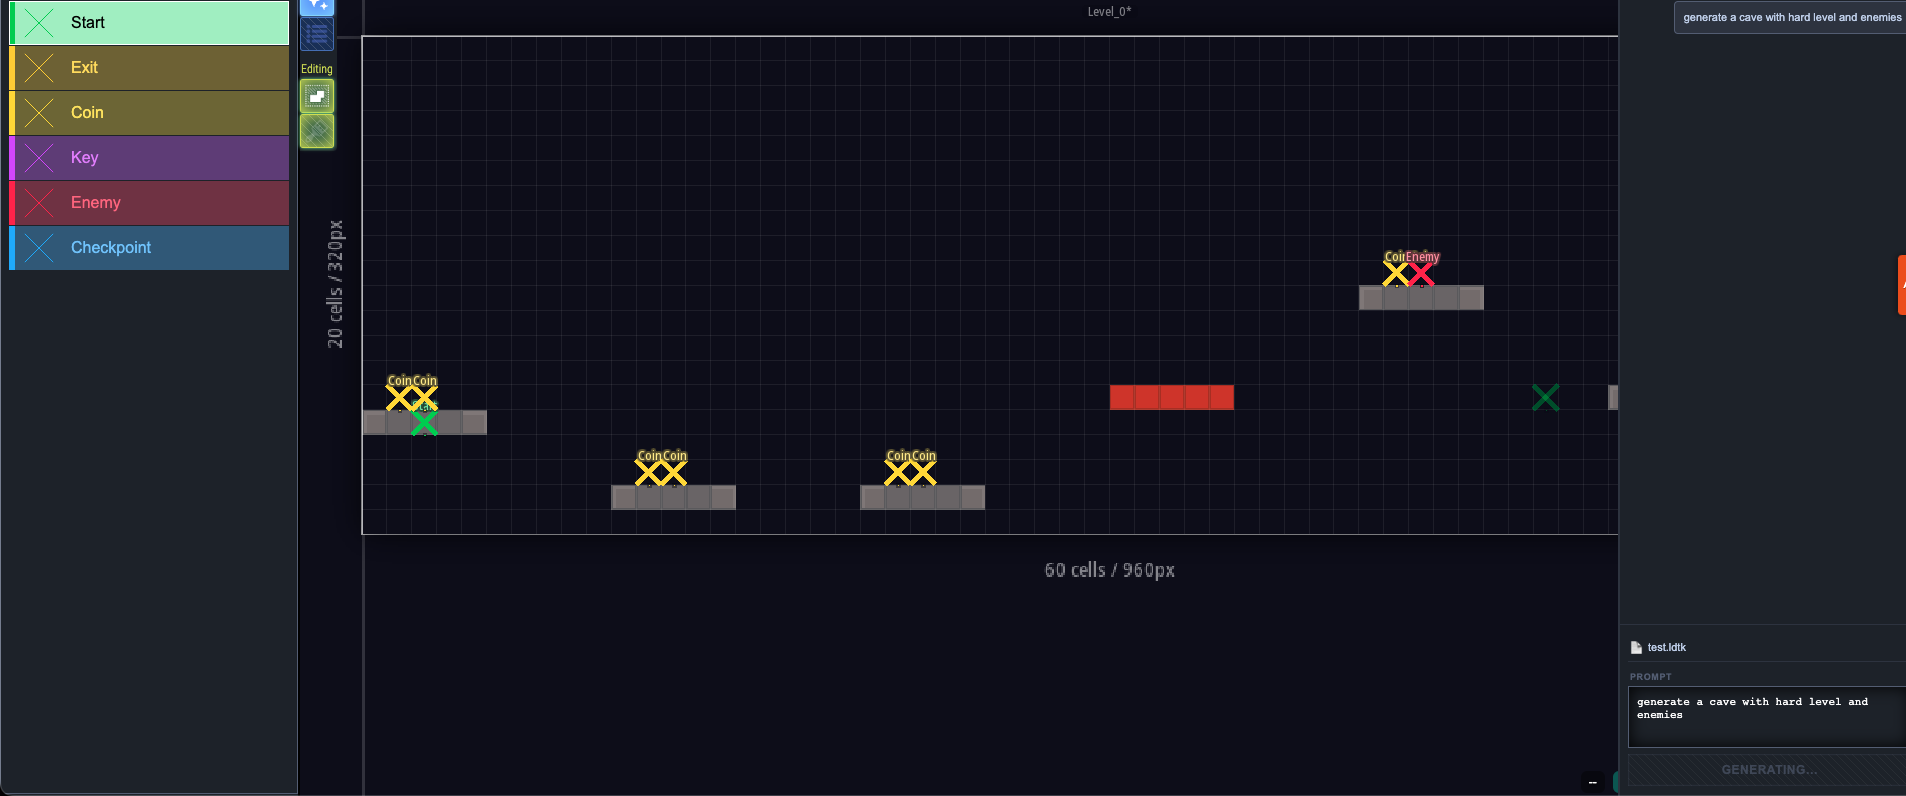
\includegraphics[width=0.72\textwidth]{figures/fig_v1_prototype.png}
\caption{The initial v1 prototype generated in LDtk: isolated 1-tile-thick floating platforms embedded in empty space via Sugiyama layered graph drawing, illustrating the structural void problem that motivated v3 rock carving.}
\label{fig:v1_prototype}
\end{figure}

\begin{enumerate}
    \item \textbf{Generation 1 (v1) --- Initial Topological Prototype:}
    The LLM generated an unconstrained directed graph (\texttt{AbstractLevelGraph}) containing nodes (\texttt{PLATFORM}, \texttt{START}, \texttt{EXIT}, \texttt{HAZARD}) and transitions (\texttt{WALK}, \texttt{JUMP}, \texttt{FALL}). Coordinates were assigned via a classical 4-phase Sugiyama layered graph drawing algorithm~\citep{sugiyama1981methods}. A basic parabolic kinematic oracle validated single jump arcs. As seen in \Cref{fig:v1_prototype}, levels produced under this generation felt like isolated platforms floating in empty air, with uniform jump costs and no surrounding architecture.
    
    \item \textbf{Generation 2 (v2) --- Grounded Specification, Grid Re-Verification \& Native UI:}
    Replaced bare graphs with a strict Pydantic v2 \texttt{LevelSpec} enforcing canvas bounds, ordered thematic sections, and a typed 9-kind entity catalog. Physics was decoupled into an external per-project \texttt{GameProfile} (\texttt{gldtk.game.json}) supporting double jumps, dashes, wall kicks, and variable gravity. GLDtk introduced rasterized grid re-verification: instead of trusting abstract graph edges, the verifier extracts actual standable spans from the raster collision grid and sweeps a $12 \times 24\text{ px}$ AABB hitbox along every physical trajectory. Mixed-initiative regional editing was integrated directly into LDtk via an Electron/Haxe sidebar (\texttt{GldtkSidebar.hx}).
    
    \item \textbf{Generation 3 (v3) --- Procedural Rock Carving, Comfort Pacing \& Play Mode:}
    To eliminate the "floating void" aesthetic, v3 introduced 7 deterministic procedural structure generators (\texttt{corridor}, \texttt{parkour}, \texttt{labyrinth}, \texttt{arena}, \texttt{shaft}, \texttt{hub}, \texttt{open}) that carve traversable spaces out of solid subterranean rock with matched boundary ports. An effort-weighted routing model penalizing vertical rise over horizontal walking was added, alongside a 5-factor difficulty model, an SVG Difficulty Curve visualizer, a live Route Overlay on the LDtk canvas, and an interactive 60~Hz in-editor Play Mode.
    
    \item \textbf{Generation 4 (v4) --- Metroidvania Progression, Soft-Lock Freedom \& RAG Stamping:}
    Upgraded verification from simple reachability ($Start \to Exit$) to complete \textbf{soft-lock freedom} via Tarjan SCC condensation and a bounded Inventory-State Product Automaton ($\mathcal{S} = V_{\text{standable}} \times \mathcal{P}(\text{Items})$). Integrated Dormans-style mission grammars~\citep{dormans2010adventures} for lock-and-key loops and ability gates. Established a 3,577-record RAG pattern library extracted from open-source games (\emph{SuperTux}, \emph{Open Surge}) with multimodal Vision-Language Model labeling and cross-project Design Memory.
\end{enumerate}

% -----------------------------------------------------------------------------
% CHAPTER 2: PROBLEM STATEMENT & ENGINEERING CHALLENGES
% -----------------------------------------------------------------------------
\chapter{Problem Statement and Engineering Failure Modes}
\label{chap:problems}

\section{Formal Problem Formulation}
Let a 2D platformer level be defined as a tuple:
\begin{equation}
    \mathcal{L} = \langle W, H, C, \mathcal{T}, \mathcal{E}, \mathcal{P}_{\text{game}} \rangle
\end{equation}
where $W, H \in \mathbb{N}$ represent the level dimensions in discrete grid tiles (with cell size $s = 16\text{ px}$), $C \in \{0, 1, 2\}^{W \times H}$ is the discrete collision matrix ($0 = \text{AIR}$, $1 = \text{ROCK}$, $2 = \text{SPIKE}$), $\mathcal{T} \in \mathbb{N}^{W \times H}$ is the visual autotile index matrix, $\mathcal{E} = \{(k_i, x_i, y_i)\}_{i=1}^m$ is the set of placed entities with catalog types $k_i \in \mathcal{K}_{\text{catalog}}$, and $\mathcal{P}_{\text{game}} = \langle g, v_{\text{run}}, v_{\text{jump}}, \mathcal{A}_{\text{abilities}}, \mathbf{h}_{\text{hitbox}} \rangle$ is the active player kinematic profile.

Given a user prompt $\mathbf{p}_{\text{user}}$ and target difficulty $\delta^* \in [0, 10]$, the level design objective is to generate $\mathcal{L}$ such that:
\begin{enumerate}
    \item \textbf{Reachability:} An unbroken, collision-free trajectory exists from the Start entity to the Exit entity under the kinematic equations of $\mathcal{P}_{\text{game}}$.
    \item \textbf{Soft-Lock Freedom:} For every reachable state $(u, I)$ where $u$ is a standable platform and $I \subseteq \mathcal{K}_{\text{items}}$ is the collected inventory, there exists a valid sequence of kinematic transitions leading to an Exit state.
    \item \textbf{Prompt Fidelity:} All explicit entity, thematic, and structural constraints specified in $\mathbf{p}_{\text{user}}$ are satisfied ($\text{Fidelity} \ge 0.95$).
    \item \textbf{Difficulty Convergence:} The measured difficulty metric $|\delta(\mathcal{L}) - \delta^*| \le 1.5$.
\end{enumerate}

\section{Ten Critical Engineering Failure Modes and Architectural Solutions}
During the evolution of GLDtk from v1 through v4, ten critical engineering failure modes were systematically identified, analyzed, and resolved (\Cref{tab:ten_issues}).

\begin{table}[htbp]
\centering
\small
\caption{Comprehensive breakdown of the ten critical failure modes encountered during GLDtk development and their engineered architectural solutions.}
\label{tab:ten_issues}
\begin{tabularx}{\textwidth}{l p{3.2cm} p{4.2cm} X}
\toprule
\textbf{\#} & \textbf{Observed Failure Mode} & \textbf{Root Cause} & \textbf{Architectural Solution} \\
\midrule
\textbf{1} & Levels felt like "floating parkour in a void" (v1--v2) & Sugiyama layout and early placement plotted isolated 1-tile platforms in empty space without enclosing geography. & \textbf{Procedural Rock Carvers (\texttt{layout/terrain/}):} 7 procedural generators carve chambers, corridors, and vaults from solid rock with aligned boundary ports. \\
\addlinespace
\textbf{2} & Floaty, unnatural 11.5-tile jumps (v1--v3) & Default physics ($g=980, v=600$) produced huge 11.5-tile arcs; uniform graph weights made 1 giant leap cheaper than 3 hops. & \textbf{Tightened Kinematics \& Comfort Pass:} Retuned to $g=1800, v=500, v_x=220$ ($\approx 4.3$-tile rise); added superlinear jump effort and comfort limits ($\text{hop}\le 4, \text{rise}\le 3$). \\
\addlinespace
\textbf{3} & LLM omitted requested entities or counts (M1) & On an 11-requirement prompt, \texttt{gemini-3.1-flash-lite} parsed requirements in JSON but emitted only 5 entities. & \textbf{Deterministic Completeness Fill (\texttt{fidelity/fill.py}):} Synthesizes missing entities, hazards, and structure keys algorithmically before layout ($\le 1$ re-prompt). \\
\addlinespace
\textbf{4} & Standable spans under 1-tile ceilings \& gravity bugs & Surface detection checked floor tiles without checking if the $12\times 24\text{ px}$ player fit upright; cross-section arcs used single $g$. & \textbf{Headroom Splitting \& Gravity Integral:} Splits spans wherever $\lceil h_{\text{hitbox}}/16 \rceil = 2$ empty tiles are missing; integrates path-moment gravity $G = 2\int_0^1 (1-\sigma)g(x(\sigma))d\sigma$. \\
\addlinespace
\textbf{5} & Traps in pits or behind locked doors & Reachability checks only verified that \emph{some} path existed, ignoring one-way drops past required keys. & \textbf{Tarjan SCC Condensation \& Product Automaton:} Verifies backward liveness over $V_{\text{standable}} \times \mathcal{P}(\text{Items})$; repairs traps with stepping stones. \\
\addlinespace
\textbf{6} & Sparse canvases \& entity crowding on 3-tile ledges & LLMs placed 8 platforms across a $120\times 30$ grid and stacked coins, bats, and checkpoints onto single ledges. & \textbf{Crowding Relocation \& Chebyshev Densification:} Enforces $\le 1$ entity per 2 tiles; infills empty air outside protected route arcs via 2D Chebyshev distance transforms. \\
\addlinespace
\textbf{7} & Gemini Free-Tier 429 quota \& 503 high-demand halts & Free tier caps Flash at $\sim 20$ requests/day and returns HTTP 503 \texttt{UNAVAILABLE} during traffic spikes. & \textbf{Multi-Tier Provider Cascades \& Exponential Backoff:} Retries 503s at 20s, 60s, 120s; cascades Gemini $\to$ Claude $\to$ local \texttt{ollama:qwen2.5:14b}. \\
\addlinespace
\textbf{8} & Local \texttt{qwen2.5:14b} failed 6/6 prompts (0\% pass) & Qwen emitted complexity on a $0\dots 10$ scale, placed entities on hazards, and labeled steep climbs as \texttt{Walk}. & \textbf{Symbolic Normalizer \& Partial Patching (PR \#7):} Normalizes bounds, rescales complexity, reclassifies steep edges---boosting replay pass rate to \textbf{83.3\% (5/6)}. \\
\addlinespace
\textbf{9} & LDtk canvas blank on reload, washed-out tiles, dirty \texttt{*} & \texttt{App.loadProject} race-disposed active editor; layer order mismatched \texttt{JSON\_SCHEMA.json}, triggering \texttt{Level.tidy()}. & \textbf{In-Place Project Swapping \& Schema Alignment:} Corrected layer order (\texttt{Entities $\to$ Tiles $\to$ Collisions}), pre-populated cached pixel buffers, swapped via \texttt{ProjectLoader}. \\
\addlinespace
\textbf{10} & RAG stamping failed on tall sections \& rare types & Pattern index lacked tall labyrinth/arena windows; 20-row windows broke when stretched across 40-row sections. & \textbf{Geometry Classifier \& Route-Checked Rock Padding:} Ingested +641 gap windows; padded stamps with rock instead of stretching; enforced verified traversal ($4/4$ coverage). \\
\bottomrule
\end{tabularx}
\end{table}

% -----------------------------------------------------------------------------
% CHAPTER 3: RELATED WORK & THEORETICAL SOURCES
% -----------------------------------------------------------------------------
\chapter{Related Work and Theoretical Foundations}
\label{chap:related}

\section{Taxonomy of Procedural Content Generation in Games}
GLDtk synthesizes literature across five distinct research domains:
\begin{enumerate}
    \item \textbf{Foundational PCG and Search-Based Methods:} Shaker et al.~\citep{shaker2016procedural} categorize PCG into constructive methods (single-pass, unverified) and search-based methods~\citep{togelius2011search}. Short and Adams~\citep{short2017procedural} detail procedural pacing, room-chunk composition, and boundary port alignment in commercial level design. While genetic algorithms require thousands of complete game simulations, GLDtk achieves real-time generation by deploying an analytical, closed-form kinematic oracle ($\mathcal{O}(1)$ evaluation per jump) paired with a closed-loop complexity controller. Summerville et al.~\citep{summerville2018pcgml} survey Procedural Content Generation via Machine Learning (PCGML), identifying that statistical models trained on raw tile matrices inevitably produce broken mechanics due to an absence of physical inductive bias.
    
    \item \textbf{LLM-Based Level Generation (2023--2026):} Sudhakaran et al.~\citep{sudhakaran2023mariogpt} introduced MarioGPT, fine-tuning GPT-2 to output text-conditioned tile columns for \emph{Super Mario Bros.} Because MarioGPT operates autoregressively on raw ASCII characters, it frequently emits impassable gaps or severed pipes, requiring post-hoc A* pathfinding to filter valid levels. Todd et al.~\citep{todd2023level} demonstrated that off-the-shelf LLMs exhibit severe spatial blindness in 2D puzzle games such as \emph{Sokoban}. Nasir et al.~\citep{nasir2024word2world} developed Word2World, generating narrative-driven top-down RPG rooms. Taveekitworachai et al.~\citep{taveekitworachai2023chatgpt4pcg, taveekitworachai2024chatgpt4pcg} established the ChatGPT4PCG benchmark, demonstrating the brittleness of prompt-to-structure synthesis in physics-based games. GLDtk extends this paradigm to 2D side-scrolling platformers with vertical gravity, replacing raw tile emission with strict JSON schema decoding and deterministic symbolic patching.
    
    \item \textbf{Constraint-Based and Mission-Space Systems:} Dormans~\citep{dormans2010adventures} and Dormans and Bakkes~\citep{dormans2011generating} established the separation between \textbf{Mission Graphs} (abstract task orderings generated via graph-rewriting grammars) and \textbf{Space Graphs} (physical room topology). GLDtk directly implements Dormans' mission-space separation in its \texttt{mission/} subsystem. Gumin's WaveFunctionCollapse (WFC)~\citep{gumin2016wave} and its constraint-solving analysis by Karth and Smith~\citep{karth2017wavefunctioncollapse} enforce local tile adjacency consistency, but cannot guarantee global kinematic reachability. Smith et al.~\citep{smith2011tanagra, smith2011launchpad} introduced Tanagra and Launchpad, pioneering mixed-initiative platformer design with reactive jump constraints. While Tanagra arranged sequences of 1D floating rectangles for a single Mario jump, GLDtk carves enclosed 2D architectural chambers and verifies multi-ability player locomotion. Cooper's Sturgeon~\citep{cooper2022sturgeon} compiled level constraints into SAT/SMT solvers; GLDtk avoids exponential SAT solving times by resolving kinematics analytically and proving soft-locks in linear time ($\mathcal{O}(V+E)$).
    
    \item \textbf{Graph Drawing and Kinematic Reachability:} Sugiyama et al.~\citep{sugiyama1981methods} formalized the 4-phase layered DAG layout algorithm adapted in GLDtk v1. Bauer et al.~\citep{bauer2013automated} utilized reachability trees to mutate local platform placement, a concept generalized by GLDtk's deterministic stepping-stone synthesis.
    
    \item \textbf{Mixed-Initiative Co-Creativity and Production Editors:} Liapis et al.~\citep{liapis2013sentient} pioneered real-time playability and difficulty heatmaps in Sentient Sketchbook. Guzdial et al.~\citep{guzdial2019morai} explored co-creative design roles in Morai Maker, finding that human designers reject generative systems that overwrite their manual modifications. GLDtk enforces non-destructive co-creativity via seam-locked regional regeneration and operationalizes the co-creative "Student" role through its cross-project Design Memory. Sébastien Bénard's work on LDtk~\citep{benard2020ldtk} and the procedural level architecture of \emph{Dead Cells}~\citep{benard2017deadcells} directly inspired GLDtk's hybrid strategy of combining macro mission graphs with micro RAG pattern stamps inside LDtk.
\end{enumerate}

\section{Eight-Dimension Comparative Evaluation Matrix}
\Cref{tab:comparison} positions GLDtk against the state of the art across eight foundational dimensions of procedural and mixed-initiative level generation.

\begin{table}[htbp]
\centering
\small
\caption{Comparative evaluation matrix contrasting GLDtk against prevailing level design paradigms across eight fundamental technical dimensions.}
\label{tab:comparison}
\begin{tabularx}{\textwidth}{l p{2.2cm} p{2.4cm} p{2.4cm} p{2.2cm} X}
\toprule
\textbf{Evaluation Dimension} & \textbf{Pure LLMs} \newline \citep{sudhakaran2023mariogpt, todd2023level} & \textbf{Constraint Solvers} \newline \citep{smith2011tanagra, cooper2022sturgeon} & \textbf{Academic UIs} \newline \citep{liapis2013sentient, guzdial2019morai} & \textbf{Manual Editors} \newline \citep{benard2020ldtk} & \textbf{GLDtk} \newline (This Thesis) \\
\midrule
\textbf{Natural Language Control} & High (free-form text) & None (code / rules) & None (brush sketching) & None (manual painting) & \textbf{Full} (prompts for levels, regions, entities) \\
\addlinespace
\textbf{Playability Proof} & None (frequent broken gaps) & High (solver bound) & Partial (heuristic simulation) & None (manual QA) & \textbf{100\% Proven} (swept-hitbox physics oracle) \\
\addlinespace
\textbf{Soft-Lock Freedom} & None (unmonitored pits) & Partial (mission-only) & None & None (manual playtest) & \textbf{Guaranteed} (Tarjan SCC + Product Graph) \\
\addlinespace
\textbf{Multi-Ability Physics} & None & Single jump only & Coarse / abstract & Manual mental math & \textbf{Full} (double jump, dash, wall kick, gravity) \\
\addlinespace
\textbf{Non-Destructive Editing} & None (re-rolls whole level) & Limited infilling & Can overwrite user work & Native manual brush & \textbf{Seam-Locked Co-Creation} (region/section) \\
\addlinespace
\textbf{Mission / Key-Lock Loops} & Weak long-horizon reasoning & High (Dormans grammars) & None & Manual wiring & \textbf{Dual Mission + Space Embedding} \\
\addlinespace
\textbf{Learns Designer Taste} & Stateless & Static weights & Session-only & None (passive tool) & \textbf{Design Memory} (learns from hand edits) \\
\addlinespace
\textbf{Studio Tool Integration} & None (CLI / ASCII scripts) & Standalone prototypes & Standalone research GUI & Native desktop application & \textbf{Native Haxe Sidebar in LDtk 1.5.3} \\
\bottomrule
\end{tabularx}
\end{table}

\section{Open-Source Licensing and Legal Risk Assessment}
Academic PCG literature heavily relies on the Video Game Level Corpus (VGLC)~\citep{summerville2016vglc}. However, VGLC platformer datasets are extracted from commercial Nintendo ROM files (\emph{Super Mario Bros.}, \emph{The Legend of Zelda}, \emph{Metroid}). Distributing level generators or pattern libraries derived from proprietary ROM data exposes commercial game studios to severe copyright and DMCA liability under international intellectual property law.

Furthermore, popular open-source games such as \emph{Frogatto \& Friends} license their level data under Creative Commons Attribution-NonCommercial-ShareAlike (CC-BY-NC-SA 3.0). The NonCommercial (NC) restriction prevents commercial studios from deploying tools derived from this corpus.

GLDtk establishes a \textbf{100\% commercially safe and legally unencumbered asset stack}:
\begin{itemize}
    \item \textbf{Tilesets and Sprites:} Curated from Kenney CC0 1.0 Public Domain packages (\emph{Tiny Dungeon}, \emph{Tiny Town}, \emph{1-Bit Pack}), providing 8 autotile themes and 25 packed entity sprites.
    \item \textbf{RAG Room Windows:} 3,336 pattern windows extracted strictly from \emph{SuperTux} (CC-BY-SA 4.0), \emph{Open Surge} (CC-BY 3.0/4.0), and official MIT-licensed LDtk samples, with full attribution metadata exposed programmatically via \texttt{GET /patterns/attribution}.
\end{itemize}

% -----------------------------------------------------------------------------
% CHAPTER 4: SYSTEM ARCHITECTURE & METHODOLOGY
% -----------------------------------------------------------------------------
\chapter{Neuro-Symbolic System Architecture and Mathematical Formulations}
\label{chap:arch}

\section{The End-to-End 11-Stage Pipeline}
The core generation pipeline (\texttt{build\_level} in \texttt{pipeline/level.py}) executes 11 deterministic and neural-guided stages (\Cref{fig:pipeline_tikz}).

\begin{figure}[htbp]
\centering
\begin{tikzpicture}[
    node distance=0.8cm and 0.4cm,
    stage/.style={rectangle, draw=blue!80!black, fill=blue!5, rounded corners=3pt, minimum width=6.8cm, minimum height=0.75cm, font=\footnotesize, align=left},
    arr/.style={-{Stealth[scale=1.0]}, thick, color=slate!70!black}
]
    \node [stage] (s1) {\textbf{1. Prompt \& Context Assembly:} Parse prompt, load \texttt{GameProfile}, RAG patterns, Design Memory};
    \node [stage, below=of s1] (s2) {\textbf{2. LLM Controller \& Schema Validation:} Pydantic \texttt{LevelSpec} $\to$ \texttt{SymbolicPatcher} repair};
    \node [stage, below=of s2] (s3) {\textbf{3. Completeness \& Fidelity Loop:} Deduce implicit entities $\to$ Deterministic Fill ($\le 1$ retry)};
    \node [stage, below=of s3] (s4) {\textbf{4. Mission Grammar \& Space Embedding:} Lock-key cycles, ability gates, shortcut loops};
    \node [stage, below=of s4] (s5) {\textbf{5. Section Terrain Carving \& RAG Stamping:} 7 procedural carvers $+$ real-game stamps};
    \node [stage, below=of s5] (s6) {\textbf{6. Swept Hitbox Physics Verification \& Soft-Lock Repair:} Tarjan SCC liveness $+$ stone repair};
    \node [stage, below=of s6] (s7) {\textbf{7. Comfort Pass \& Chebyshev Densification:} Jump comfort limits $+$ reachable air infill};
    \node [stage, below=of s7] (s8) {\textbf{8. Closed-Loop Complexity Controller:} 5-factor difficulty model adjustment};
    \node [stage, below=of s8] (s9) {\textbf{9. Domain-Warped fBm Noise Rock Fill:} Cellular automata smoothing outside protected envelope};
    \node [stage, below=of s9] (s10) {\textbf{10. Aesthetic Autotiling Layer:} 14-role Wang autotiler, 8 CC0 themes, 25 entity sprites};
    \node [stage, below=of s10] (s11) {\textbf{11. LDtk JSON Serialization \& Native Reload:} In-place swap $\to$ Route Overlay $\to$ Play Mode};

    \draw [arr] (s1) -- (s2);
    \draw [arr] (s2) -- (s3);
    \draw [arr] (s3) -- (s4);
    \draw [arr] (s4) -- (s5);
    \draw [arr] (s5) -- (s6);
    \draw [arr] (s6) -- (s7);
    \draw [arr] (s7) -- (s8);
    \draw [arr] (s8) -- (s9);
    \draw [arr] (s9) -- (s10);
    \draw [arr] (s10) -- (s11);
\end{tikzpicture}
\caption{The 11-stage neuro-symbolic level generation pipeline implemented in GLDtk.}
\label{fig:pipeline_tikz}
\end{figure}

\section{Kinematic Physics Oracle: Mathematical Formulations}
The Physics Oracle (\texttt{symbolic/physics.py}, \texttt{symbolic/walljump.py}, \texttt{symbolic/gravity.py}) evaluates physical reachability in a Cartesian coordinate system where 1 tile equals $s = 16\text{ px}$ and $y$ increases upward.

\subsection{Standard Parabolic Jump Kinematics}
Consider a player launching from platform point $p_1 = (x_1, y_1)$ toward target landing point $p_2 = (x_2, y_2)$ with horizontal displacement $\Delta x = x_2 - x_1$ and vertical rise $\Delta y = y_2 - y_1$. Under constant downward gravity $g > 0$, maximum upward vertical impulse $v_y \in (0, v_{\text{jump}}]$, and maximum run velocity $|v_x| \le v_{\text{run}}$, the vertical equation of motion is:
\begin{equation}
    y(t) = y_1 + v_y t - \frac{1}{2} g t^2 \implies \frac{1}{2} g t^2 - v_y t + \Delta y = 0
    \label{eq:parabola}
\end{equation}
The discriminant of \Cref{eq:parabola} is:
\begin{equation}
    D = v_y^2 - 2 g \Delta y
\end{equation}

\begin{proposition}[Single Jump Feasibility]
A parabolic jump between $p_1$ and $p_2$ is kinematically feasible if and only if:
\begin{enumerate}
    \item $D \ge 0$ (the jump apex $h_{\max} = \frac{v_y^2}{2g} \ge \Delta y$).
    \item There exists a positive real flight time $t^* \in \{t_1, t_2\}$ such that:
    \begin{equation}
        \left| \frac{\Delta x}{t^*} \right| \le v_{\text{run}} + \varepsilon \quad (\varepsilon = 10^{-9})
    \end{equation}
    where $t_{1,2} = \frac{v_y \mp \sqrt{D}}{g}$.
\end{enumerate}
\end{proposition}
The descending root $t_2 = \frac{v_y + \sqrt{D}}{g}$ maximizes total airborne duration and therefore yields the maximum reachable horizontal span $|\Delta x|_{\max} = v_{\text{run}} t_2$.

\subsection{Closed-Form Double-Jump Optimal Apex Chaining}
When the player possesses the \texttt{double\_jump} ability, they can execute a second upward impulse $v_2$ at any airborne time $\tau \in [0, 2v_1/g]$ during the primary jump (initial impulse $v_1$).

At intermediate flight time $\tau$, the player's vertical elevation is:
\begin{equation}
    h(\tau) = v_1 \tau - \frac{1}{2} g \tau^2
\end{equation}
Initiating the second impulse $v_2$ at elevation $h(\tau)$ yields remaining flight time $s(\tau) = \frac{v_2 + \sqrt{D(\tau)}}{g}$, where the second-stage discriminant is:
\begin{equation}
    D(\tau) = v_2^2 + 2g(h(\tau) - \Delta y) = v_1^2 + v_2^2 - 2g\Delta y - (g\tau - v_1)^2
\end{equation}
The total airborne flight duration is $T(\tau) = \tau + s(\tau)$:
\begin{equation}
    T(\tau) = \tau + \frac{v_2 + \sqrt{v_1^2 + v_2^2 - 2g\Delta y - (g\tau - v_1)^2}}{g}
\end{equation}

\begin{theorem}[Analytical Double-Jump Apex Optimum]
The total flight time $T(\tau)$ is strictly concave over valid launch times $\tau$. Setting the first derivative $\frac{dT}{d\tau} = 0$ yields:
\begin{equation}
    \frac{dT}{d\tau} = 1 + \frac{-(g\tau - v_1)}{\sqrt{D(\tau)}} = 0 \implies \sqrt{D(\tau)} = g\tau - v_1
\end{equation}
Squaring both sides and substituting $D(\tau)$:
\begin{equation}
    v_1^2 + v_2^2 - 2g\Delta y - (g\tau - v_1)^2 = (g\tau - v_1)^2 \implies 2(g\tau - v_1)^2 = v_1^2 + v_2^2 - 2g\Delta y
\end{equation}
Solving for the optimal second-jump trigger time $\tau^*$ yields the closed-form $\mathcal{O}(1)$ expression:
\begin{equation}
    \tau^* = \min\left( \frac{v_1 + \sqrt{\frac{v_1^2 + v_2^2 - 2g\Delta y}{2}}}{g}, \;\frac{2v_1}{g} \right)
    \label{eq:double_jump_opt}
\end{equation}
\end{theorem}
This analytical result eliminates numerical optimization loops. In unit testing (\texttt{tests/test\_abilities.py}), \Cref{eq:double_jump_opt} matched 20,000 brute-force grid searches with zero divergence.

\subsection{Air Dash, Wall-Jump Climbs, and Heterogeneous Gravity}
\begin{itemize}
    \item \textbf{Horizontal Air Dash (\texttt{check\_dash\_jump}):} The player executes a burst of distance $d_{\text{dash}}$ during which vertical gravity is suspended ($g_{\text{eff}} = 0$). The oracle subtracts $d_{\text{dash}}$ from horizontal displacement ($|\Delta x|' = \max(0, |\Delta x| - d_{\text{dash}})$) and sweeps hitbox clearance across split fractions $\phi \in \{0.5, 0.0, 1.0, 0.25, 0.75\}$.
    
    \item \textbf{Wall-Jump Climbs (\texttt{symbolic/walljump.py}):} Detects continuous vertical \texttt{WallFace} boundaries ($\ge \text{player\_height}$ tiles) and executes a depth-bounded search ($\text{MAX\_KICKS} = 6$) with kick velocity $v_{\text{kick}} = \min(v_{\text{wall}}, \sqrt{2g \cdot \text{max\_climb\_px}})$.
    
    \item \textbf{Piecewise Cross-Section Gravity (\texttt{symbolic/gravity.py}):} When an airborne trajectory crosses section boundaries with distinct gravity multipliers ($g_1, g_2$), vertical displacement over total time $T$ satisfies the exact path-moment integral:
    \begin{equation}
        y(T) - y_0 = v_y T - \frac{1}{2} G T^2, \quad \text{where } G = 2 \int_0^1 (1 - \sigma) g(x_0 + \sigma \Delta x)\,d\sigma
    \end{equation}
    
    \item \textbf{Swept Hitbox Clearance:} Trajectories are sampled at discrete intervals $\Delta s \le 6.0\text{ px}$. At each sample, the player's $12 \times 24\text{ px}$ AABB bounding box is tested for intersection against solid and hazard tiles.
\end{itemize}

\section{Formal Soft-Lock Freedom via SCC Condensation and Product Automata}
A fundamental contribution of GLDtk is verifying that no player can ever become permanently stranded. Building upon Tarjan's linear-time depth-first search graph analysis~\citep{tarjan1972depth}, we formulate soft-lock verification via two complementary algorithms.

\subsection{Algorithm 1: Movement Graph SCC Liveness}
Let $G = (V_{\text{standable}}, E)$ be the extracted platform movement graph. Directed edges represent reversible walks, falls, or jump transitions.

\begin{algorithm}[H]
\caption{Tarjan SCC Condensation for Movement Trap Detection}
\label{alg:scc_softlock}
\begin{algorithmic}[1]
\Require Extracted platform movement graph $G = (V, E)$, Start node $v_{\text{start}}$, Exit nodes $V_{\text{exit}}$
\Ensure Set of unescapable trap vertices $V_{\text{trap}}$
\State Compute strongly connected components $\mathcal{C} = \text{TarjanSCC}(G)$
\State Construct condensed DAG $\mathcal{D} = (\mathcal{C}, \mathcal{E}_{\text{cond}})$ where $(C_i, C_j) \in \mathcal{E}_{\text{cond}} \iff \exists u \in C_i, v \in C_j \text{ with } (u, v) \in E$
\State Mark all components $C \in \mathcal{C}$ containing any $v \in V_{\text{exit}}$ as \textbf{Live}
\State Perform reverse topological traversal on $\mathcal{D}$: mark $C_i$ as \textbf{Live} if $\exists (C_i, C_j) \in \mathcal{E}_{\text{cond}}$ with $C_j$ \textbf{Live}
\State $V_{\text{reachable}} \gets \text{BFS}(G, v_{\text{start}})$
\State $V_{\text{trap}} \gets \emptyset$
\For{each component $C \in \mathcal{C}$}
    \If{$C$ is not \textbf{Live}}
        \State $V_{\text{trap}} \gets V_{\text{trap}} \cup (C \cap V_{\text{reachable}})$
    \EndIf
\EndFor
\State \Return $V_{\text{trap}}$
\end{algorithmic}
\end{algorithm}

If $V_{\text{trap}} \ne \emptyset$, each trap component is classified as a \texttt{pit} (entered via a one-way vertical fall) or a \texttt{sealed} chamber, and repaired algorithmically by synthesizing a chain of up to 4 stepping stones (\texttt{layout/softlock\_repair.py}).

\subsection{Algorithm 2: Bounded Inventory-State Product Automaton}
When keys, doors, and ability pickups are present, reachability depends on the player's carried inventory. Let $\mathcal{K}$ be the set of collectible items ($|\mathcal{K}| \le 6$). We define the Inventory-State Product Automaton:
\begin{equation}
    \mathcal{S} = V_{\text{standable}} \times \mathcal{P}(\mathcal{K}), \quad |\mathcal{S}| \le 64 |V_{\text{standable}}|
\end{equation}

\begin{algorithm}[H]
\caption{Inventory-State Product Automaton Model Checking}
\label{alg:product_automaton}
\begin{algorithmic}[1]
\Require Platform graph $G=(V, E)$, items $\mathcal{K}$, doors $\mathcal{D}$, Start state $s_0 = (v_{\text{start}}, \emptyset)$, Goal $V_{\text{exit}}$
\Ensure Verified soft-lock freedom or counterexample path
\State Initialize queue $Q \gets [s_0]$, visited set $\mathcal{V} \gets \{s_0\}$
\While{$Q$ is not empty}
    \State Pop $(u, I)$ from $Q$
    \For{each directed edge $(u, v) \in E$}
        \If{$v$ is obstructed by locked door $d \in \mathcal{D}$ and required key $k_d \notin I$}
            \State \textbf{continue} \Comment{Locked door gate}
        \EndIf
        \State $I' \gets I \cup \{k\}$ if platform $v$ contains collectible item $k$ else $I$
        \State $s' \gets (v, I')$
        \If{$s' \notin \mathcal{V}$}
            \State $\mathcal{V} \gets \mathcal{V} \cup \{s'\}$, Push $s'$ to $Q$
        \EndIf
    \EndFor
\EndWhile
\State Construct reverse product graph $\mathcal{S}_{\text{rev}}$ on visited states $\mathcal{V}$
\State $S_{\text{winning}} \gets \{(v, I) \in \mathcal{V} \mid v \in V_{\text{exit}}\}$
\State $S_{\text{live}} \gets \text{BFS}(\mathcal{S}_{\text{rev}}, S_{\text{winning}})$
\State $S_{\text{deadlocks}} \gets \mathcal{V} \setminus S_{\text{live}}$
\State \textbf{Assert} $S_{\text{deadlocks}} = \emptyset$
\For{each door $d$ and unlocking key $k_d$} \Comment{Counterfactual key-behind-door check}
    \State \textbf{Assert} $k_d \in \text{Reach}(G \setminus \{d\}, v_{\text{start}})$
\EndFor
\end{algorithmic}
\end{algorithm}

\section{Procedural Section Rock Carving and Stamping}
\label{sec:carvers}
GLDtk implements 7 deterministic rock carvers (\texttt{layout/terrain/}) that hollow out chambers from solid rock, maintaining aligned boundary ports (\Cref{fig:terrain_structures}):
\begin{enumerate}
    \item \textbf{Corridor:} Single-pass arterial transit with ceiling vaults and floor elevation steps.
    \item \textbf{Parkour:} Staggered jump ledges spanning spiked pits and precision hop obstacles.
    \item \textbf{Labyrinth:} Recursive backtracker maze with a $2:1$ horizontal corridor bias to ensure platformer navigability.
    \item \textbf{Arena:} Symmetrical open combat chamber with tiered observation platforms and boss staging.
    \item \textbf{Shaft:} High-aspect vertical chamber with an 11-column alternating zigzag climb.
    \item \textbf{Hub:} Central crossroads chamber supporting multi-directional branches.
    \item \textbf{Open:} Minimal perimeter boundary for free-form platform placement.
\end{enumerate}

\begin{figure}[htbp]
\centering
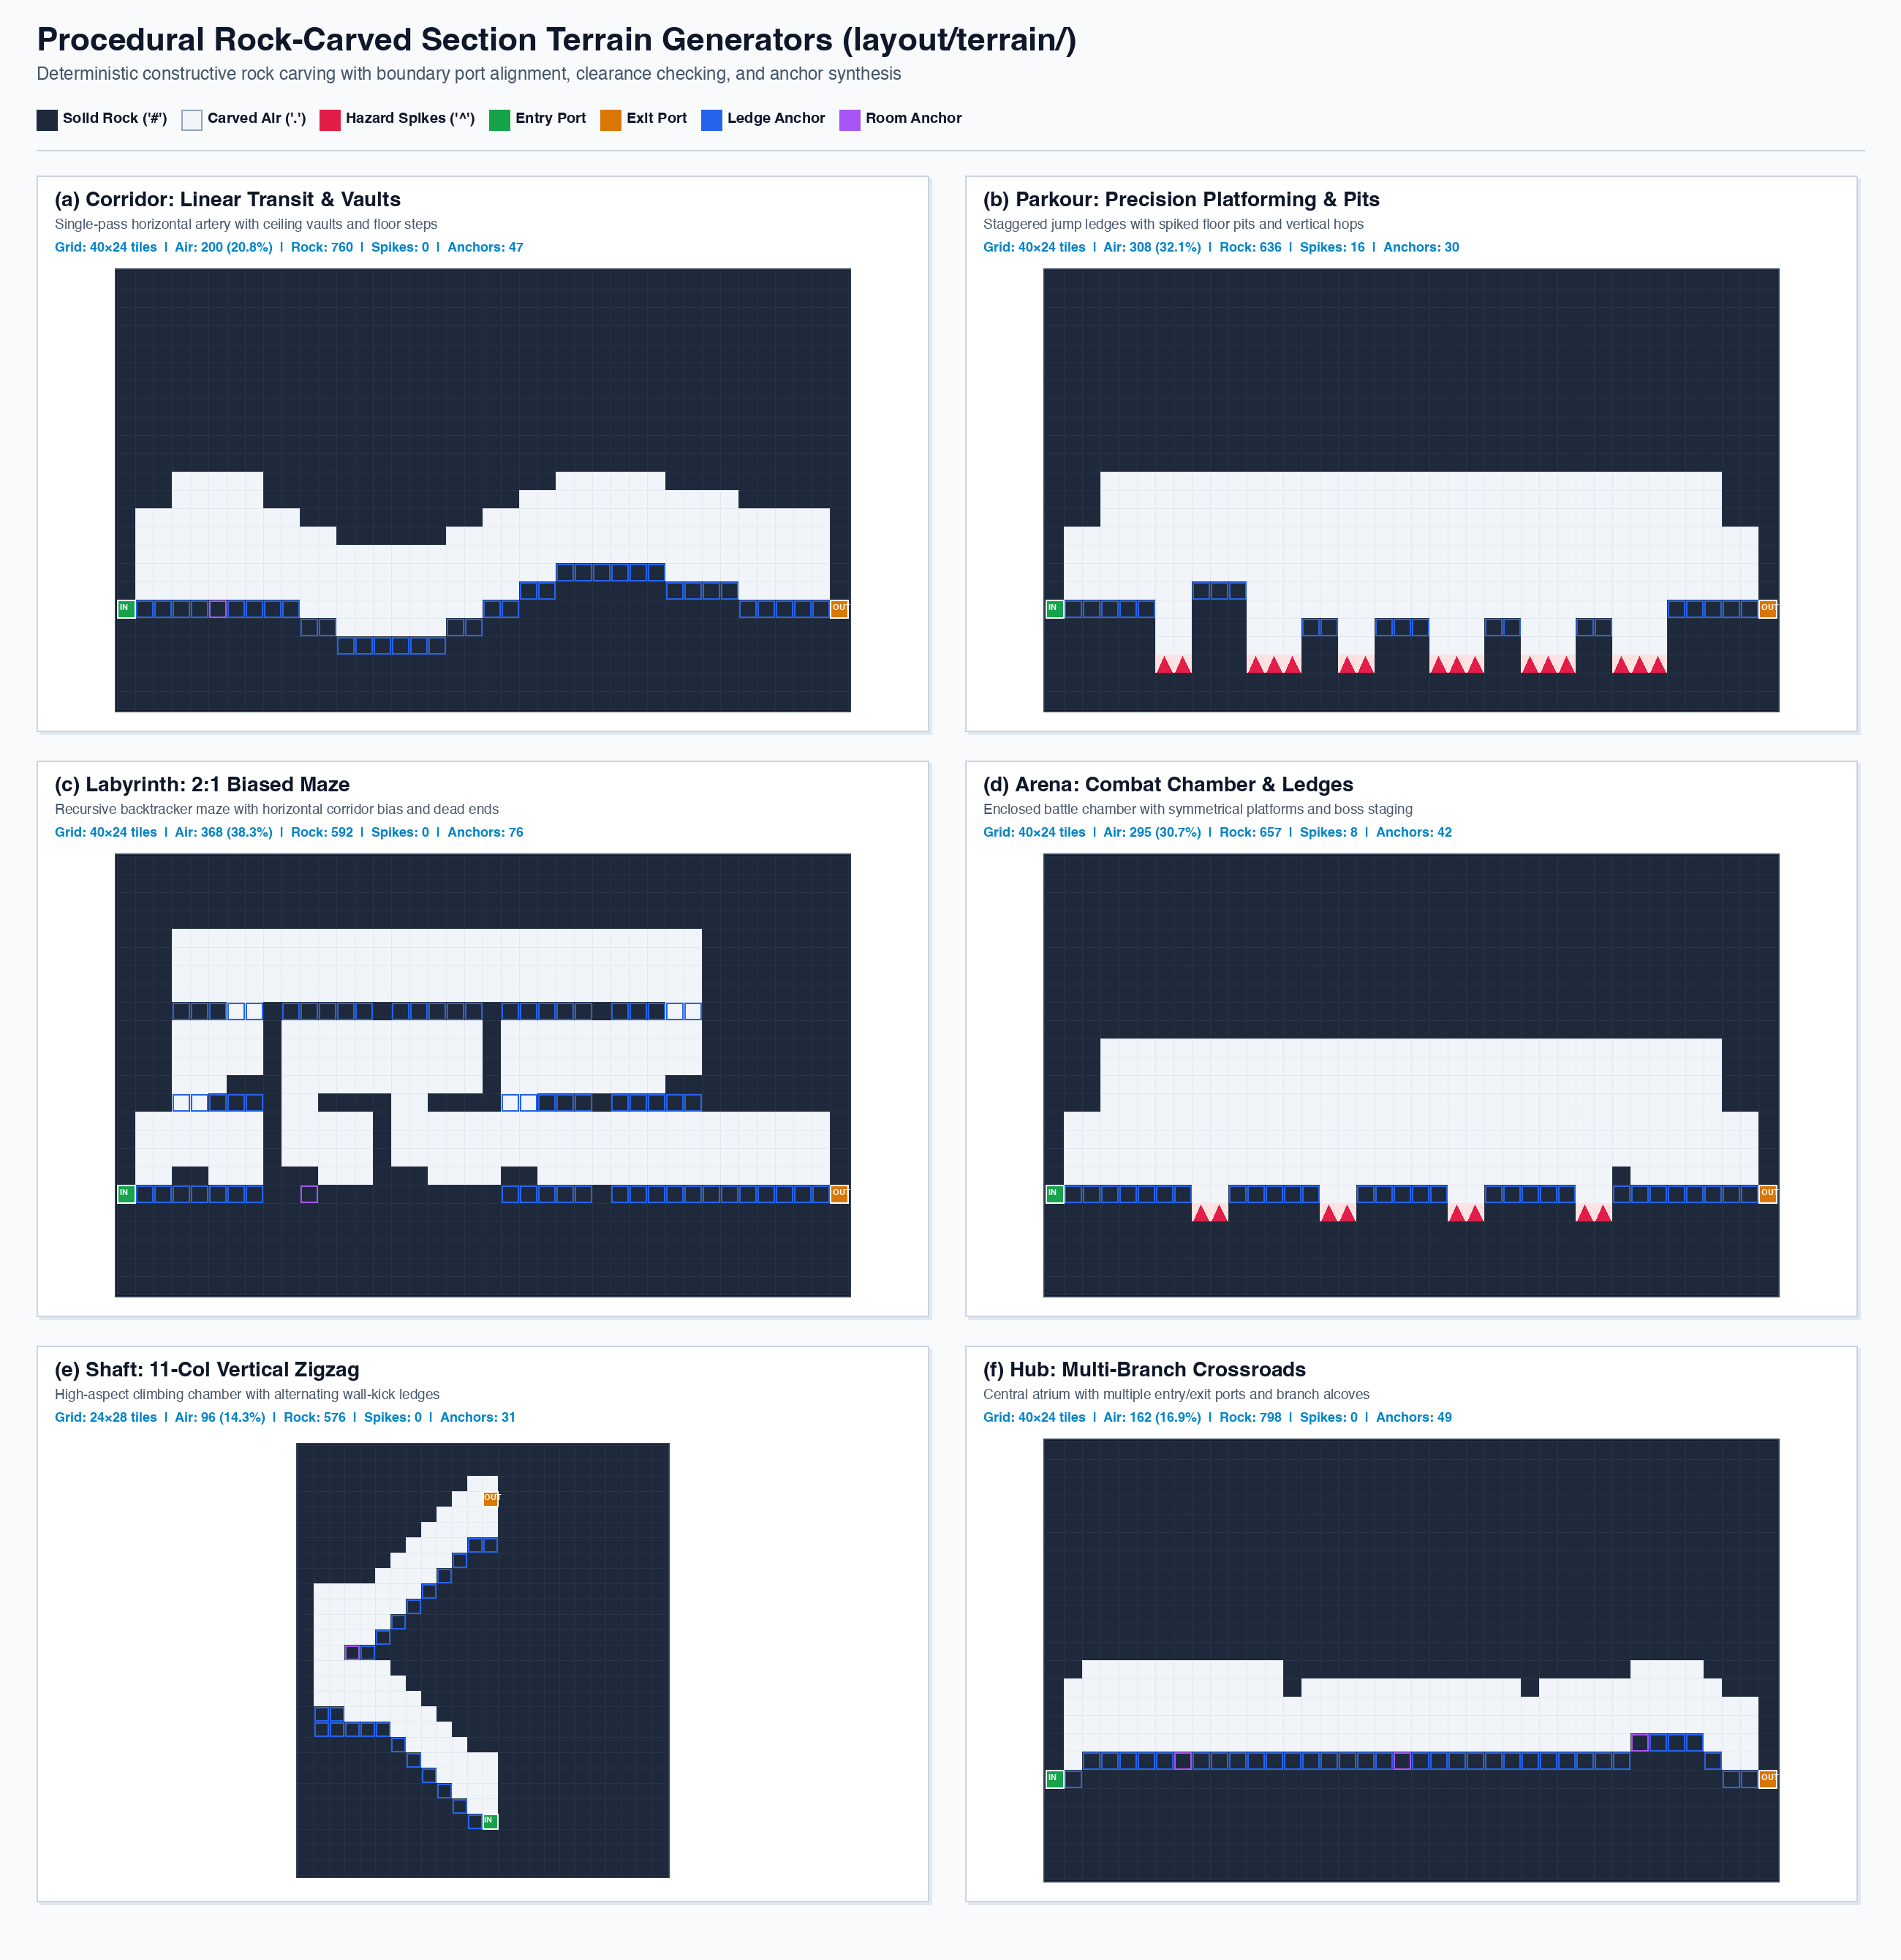
\includegraphics[width=0.98\textwidth]{figures/fig_terrain_structures.png}
\caption{Visual composite of the six primary procedural rock-carved section structures generated by \texttt{layout/terrain/}, color-coding solid rock, carved air space, hazard spikes, entry/exit ports, and semantic anchor points.}
\label{fig:terrain_structures}
\end{figure}

\section{RAG Pattern Library and Multimodal Vision Labeling}
\label{sec:vision_rag}
The RAG pattern index contains 3,577 records extracted from open-source games. To ensure semantic accuracy, GLDtk deploys a multimodal Vision-Language Model pipeline (\texttt{patterns/vision.py}). Discrete ASCII pattern windows are rasterized into color-coded PNG images (\Cref{fig:vision_pattern}) and fed to vision models (\texttt{gemini-3.5-flash-lite} or \texttt{qwen2.5vl:7b}) alongside ground-truth tile counts. A deterministic post-hoc audit flags any discrepancy between claimed and actual features, ensuring zero false claims across the entire index.

\begin{figure}[htbp]
\centering
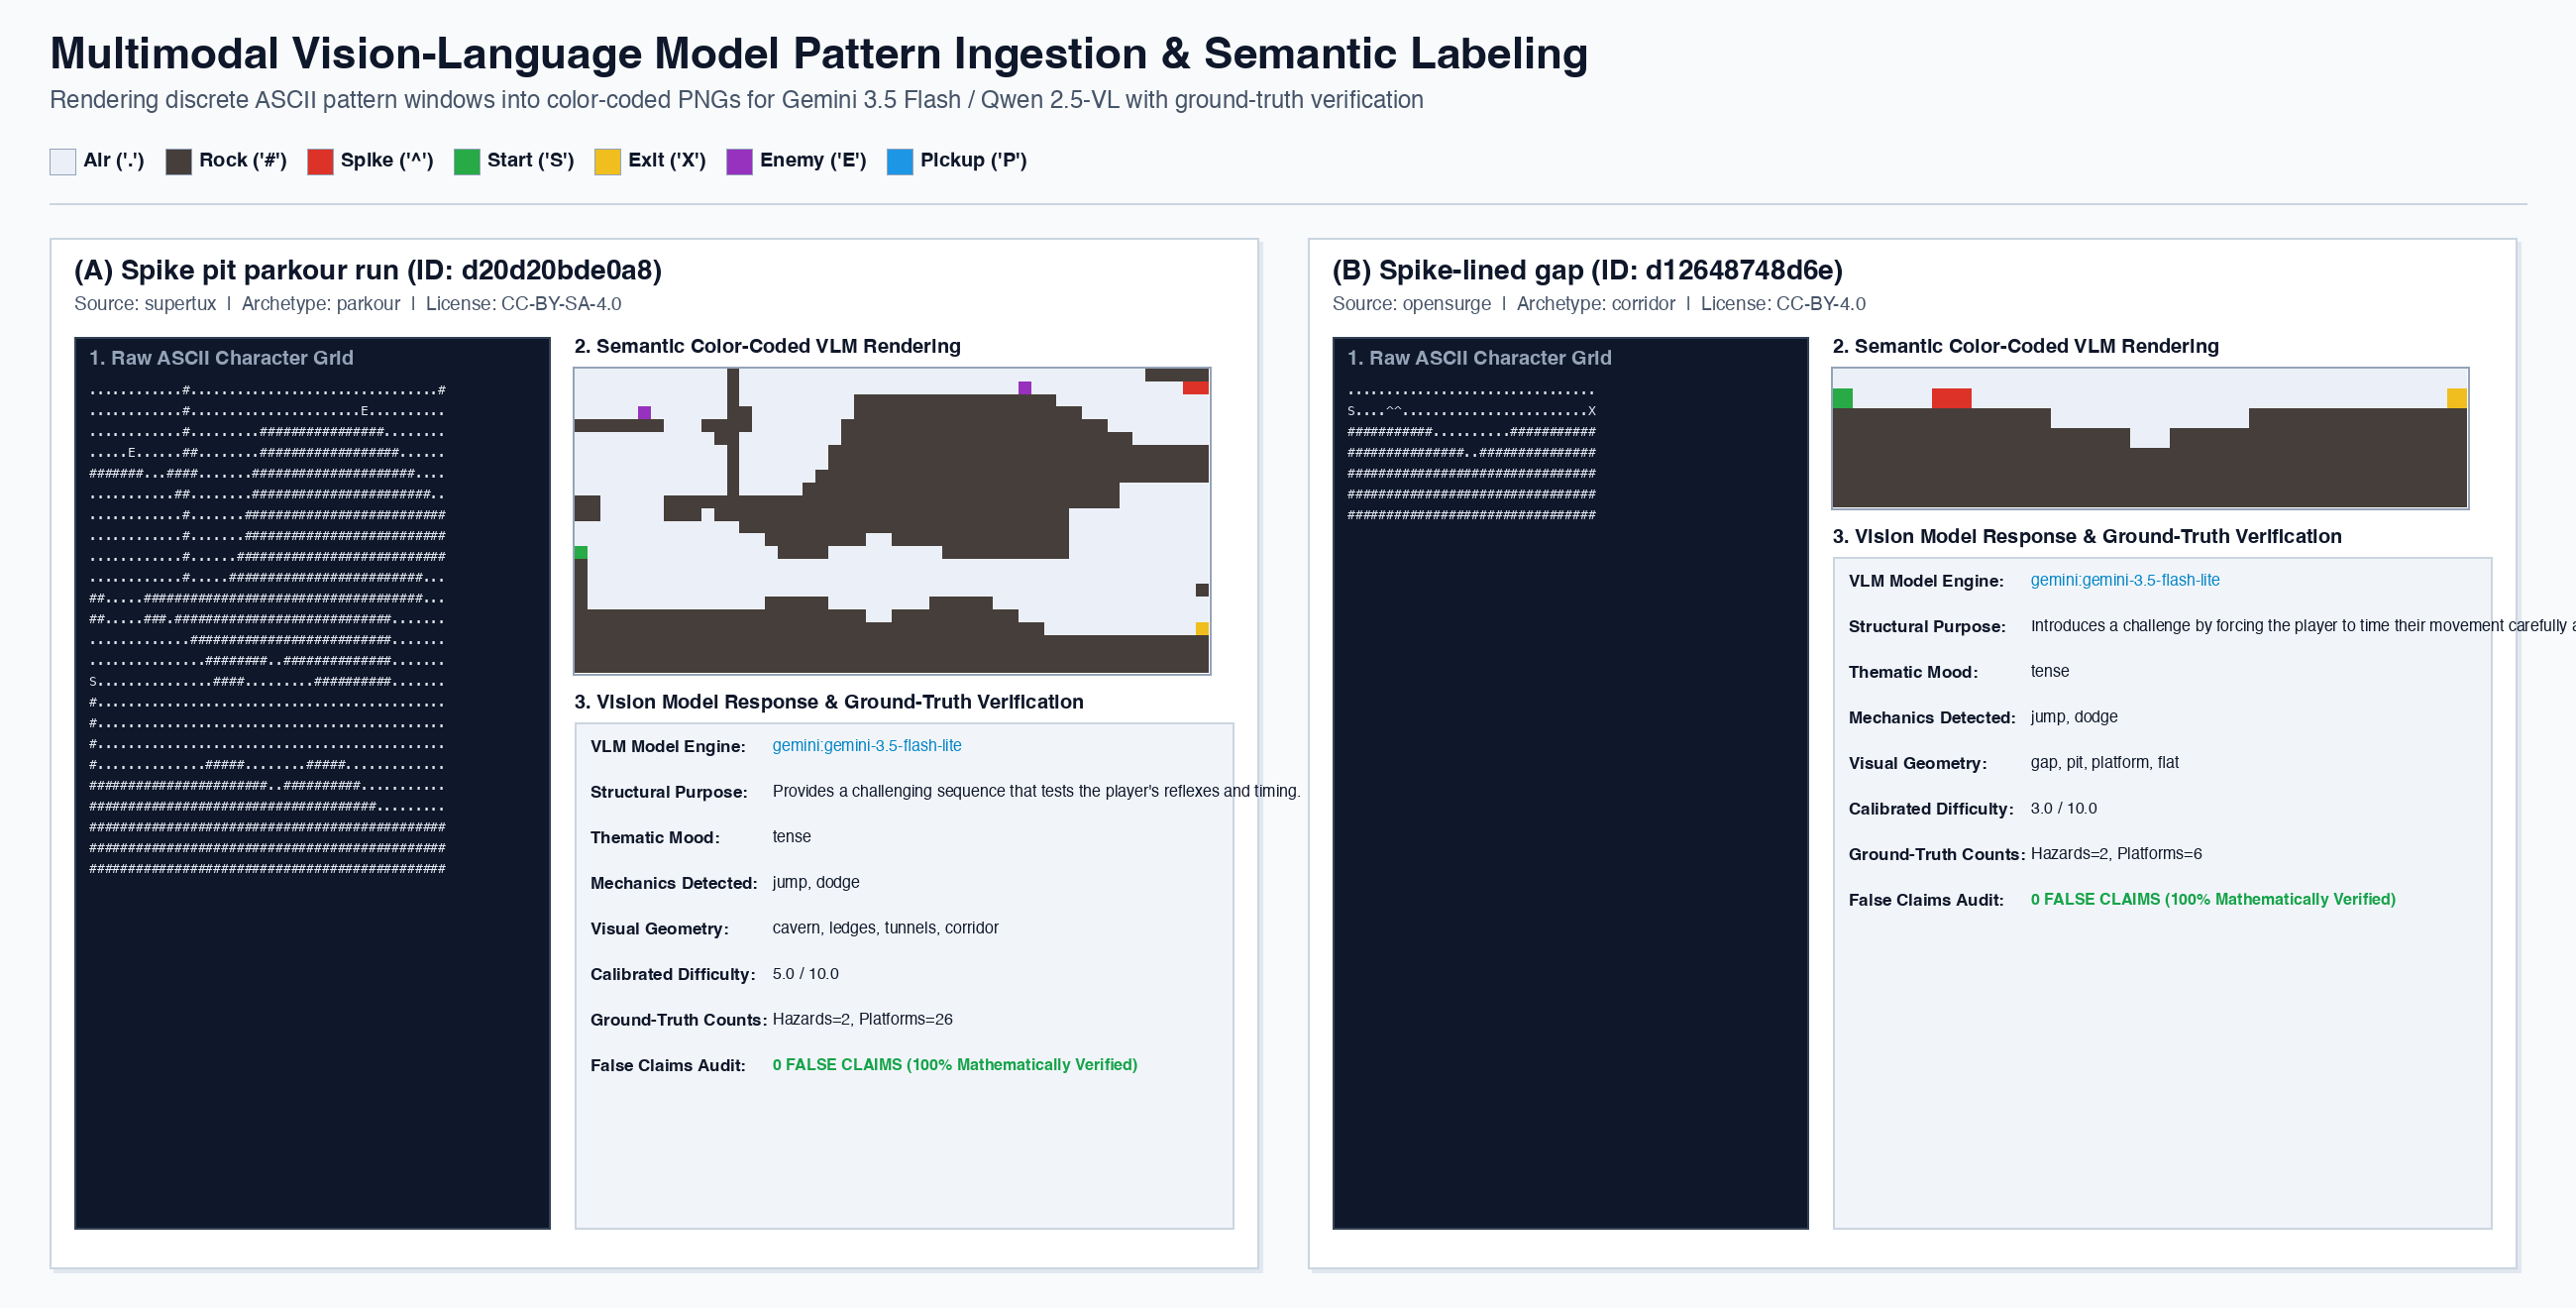
\includegraphics[width=0.98\textwidth]{figures/fig_vision_pattern.png}
\caption{Multimodal Vision-Language Model pattern ingestion pipeline, showing raw ASCII grids, semantic color-coded PNG renderings, and verified structured metadata outputs with zero false claims.}
\label{fig:vision_pattern}
\end{figure}

\section{Native LDtk Sidebar and Mixed-Initiative Workflow}
GLDtk integrates natively into LDtk 1.5.3 as an Electron/Haxe sidebar (\Cref{fig:sidebar_prompt,fig:generating_progress,fig:generated_level_route,fig:section_edit_arena,fig:after_undo,fig:asset_library}):
\begin{itemize}
    \item \textbf{Prompt \& Controls (\Cref{fig:sidebar_prompt}):} Text prompt entry, difficulty slider, rock fill toggles, RAG example selection, and multi-tier LLM provider configuration.
    \item \textbf{Live Generation Feedback (\Cref{fig:generating_progress}):} Asynchronous progress updates and responsive cancellation support.
    \item \textbf{Route Overlay \& Fidelity Report (\Cref{fig:generated_level_route}):} Visualizes the verified kinematic jump route directly on the canvas alongside a 100\% fidelity breakdown.
    \item \textbf{Mixed-Initiative Section Editing (\Cref{fig:section_edit_arena}):} Enables designers to select an existing section and transform its archetype (e.g., converting a labyrinth into an arena in 2.9s without invoking an LLM), while displaying the SVG Difficulty Curve.
    \item \textbf{Non-Destructive Undo (\Cref{fig:after_undo}):} Restores prior snapshots in under 0.8s without project reload artifacts.
    \item \textbf{Curated CC0 Asset Library (\Cref{fig:asset_library}):} 8 Kenney autotile themes and 25 packed entity sprites.
\end{itemize}

\begin{figure}[htbp]
\centering
\begin{subfigure}[b]{0.48\textwidth}
    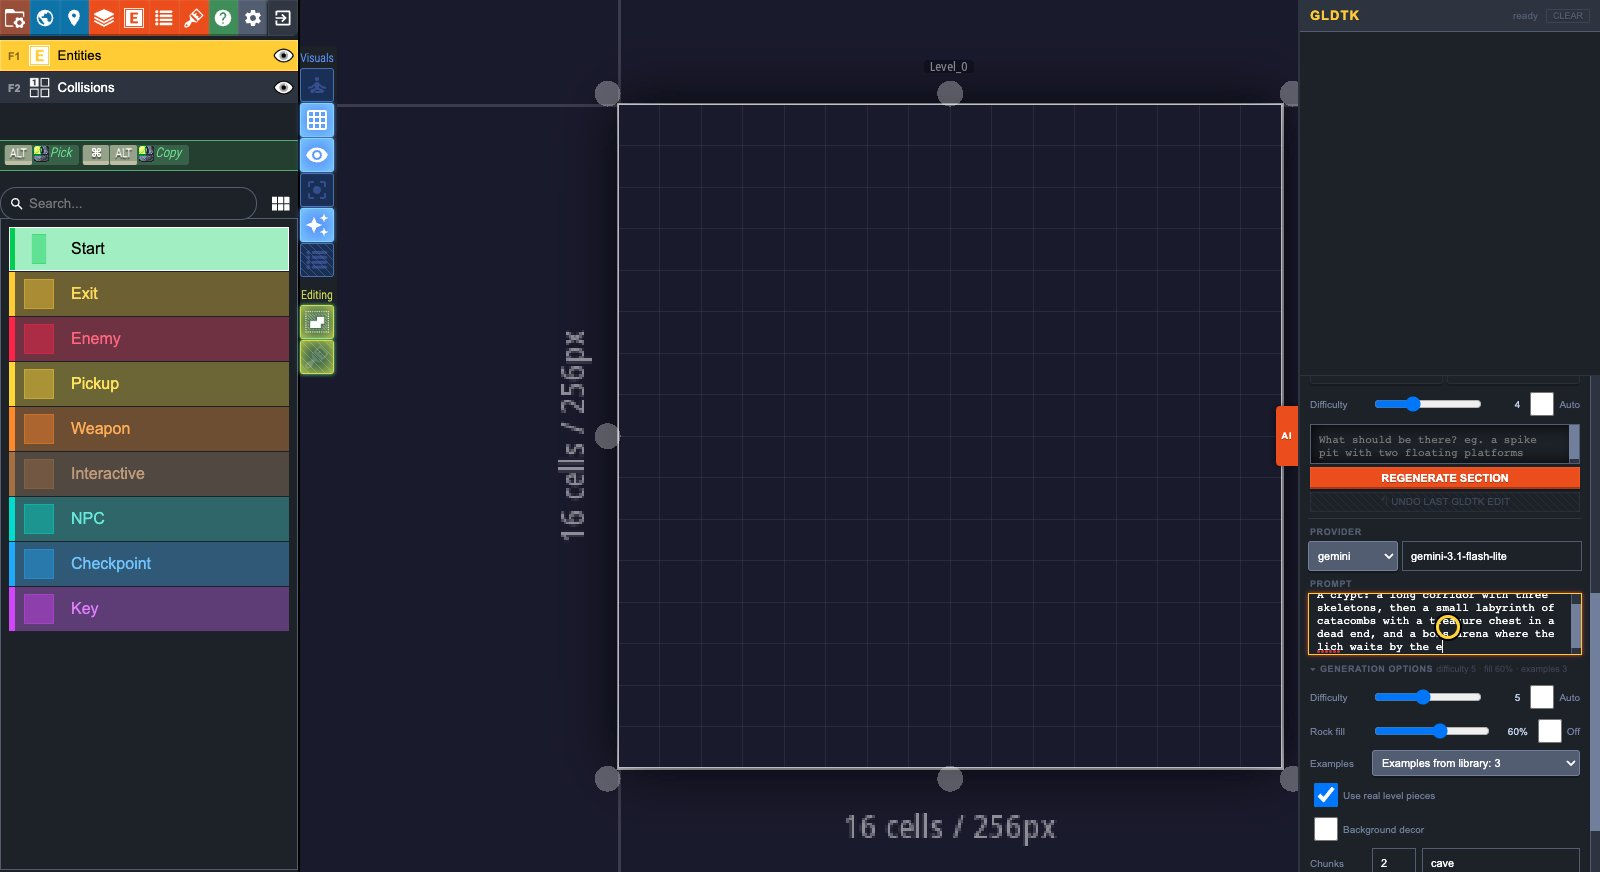
\includegraphics[width=\textwidth]{figures/fig_sidebar_prompt.jpg}
    \caption{GLDtk sidebar with prompt and provider controls.}
    \label{fig:sidebar_prompt}
\end{subfigure}
\hfill
\begin{subfigure}[b]{0.48\textwidth}
    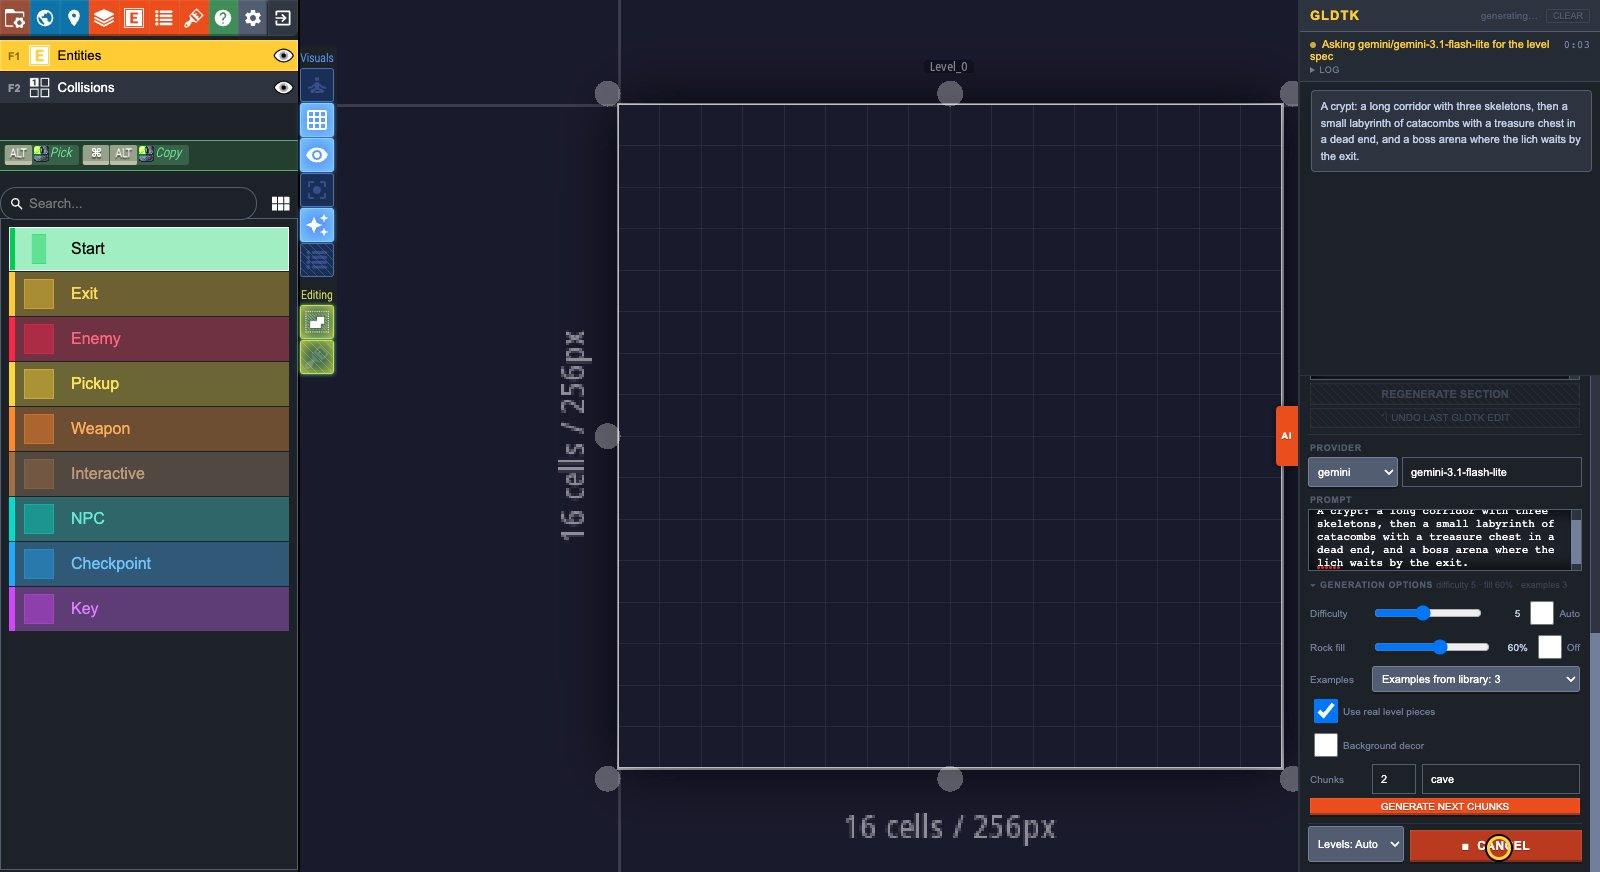
\includegraphics[width=\textwidth]{figures/fig_generating_progress.jpg}
    \caption{Live asynchronous generation progress.}
    \label{fig:generating_progress}
\end{subfigure}
\\[0.3cm]
\begin{subfigure}[b]{0.48\textwidth}
    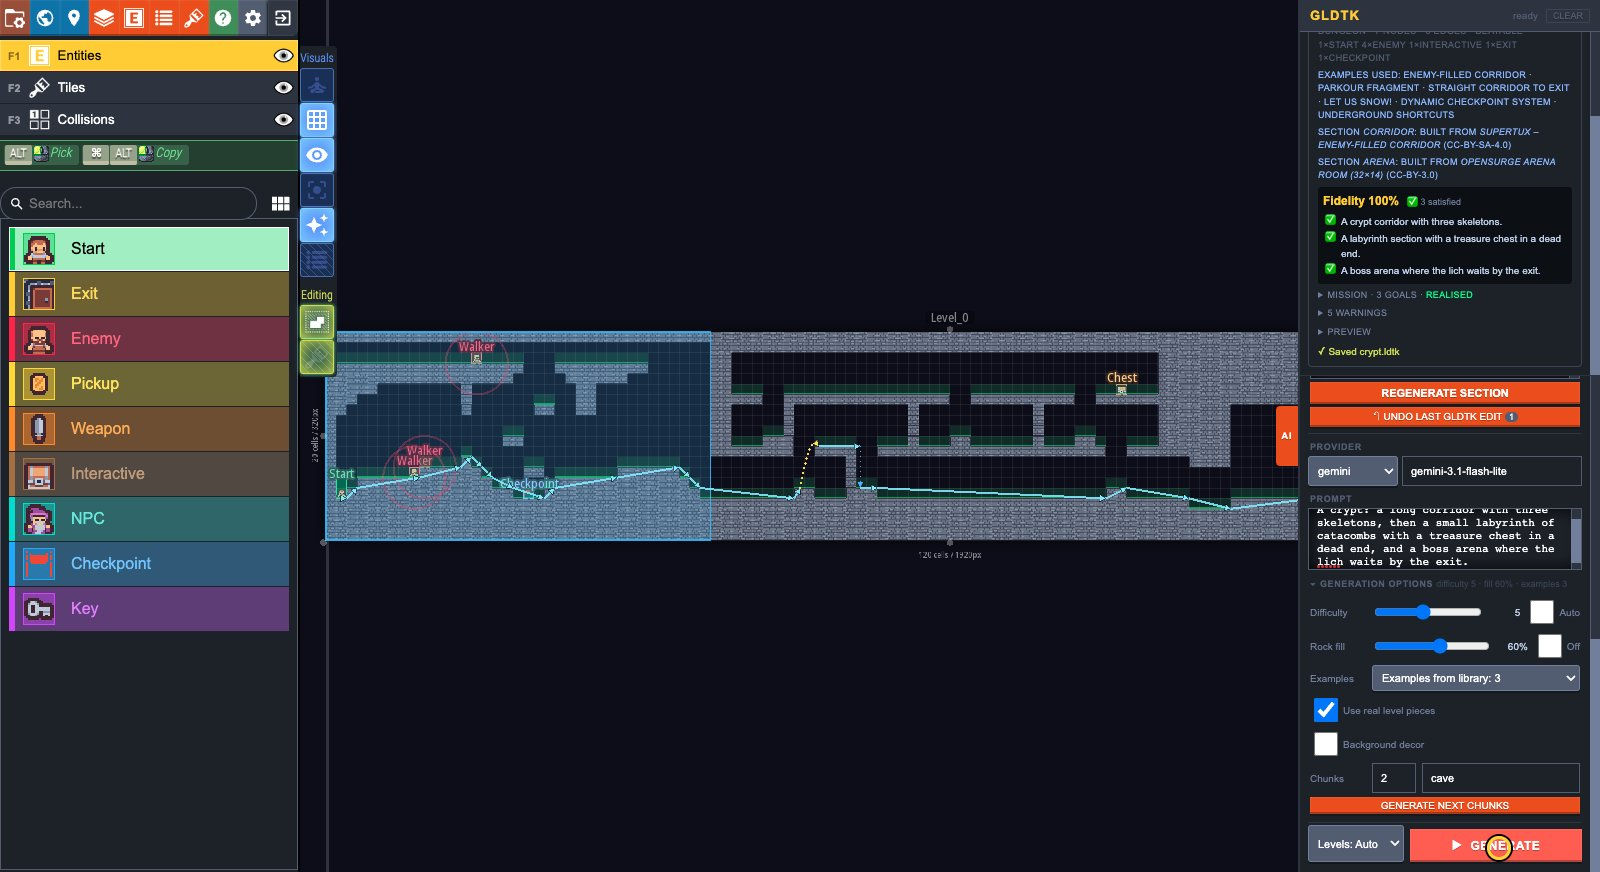
\includegraphics[width=\textwidth]{figures/fig_generated_level_route.jpg}
    \caption{Generated level with Route Overlay and Fidelity Report.}
    \label{fig:generated_level_route}
\end{subfigure}
\hfill
\begin{subfigure}[b]{0.48\textwidth}
    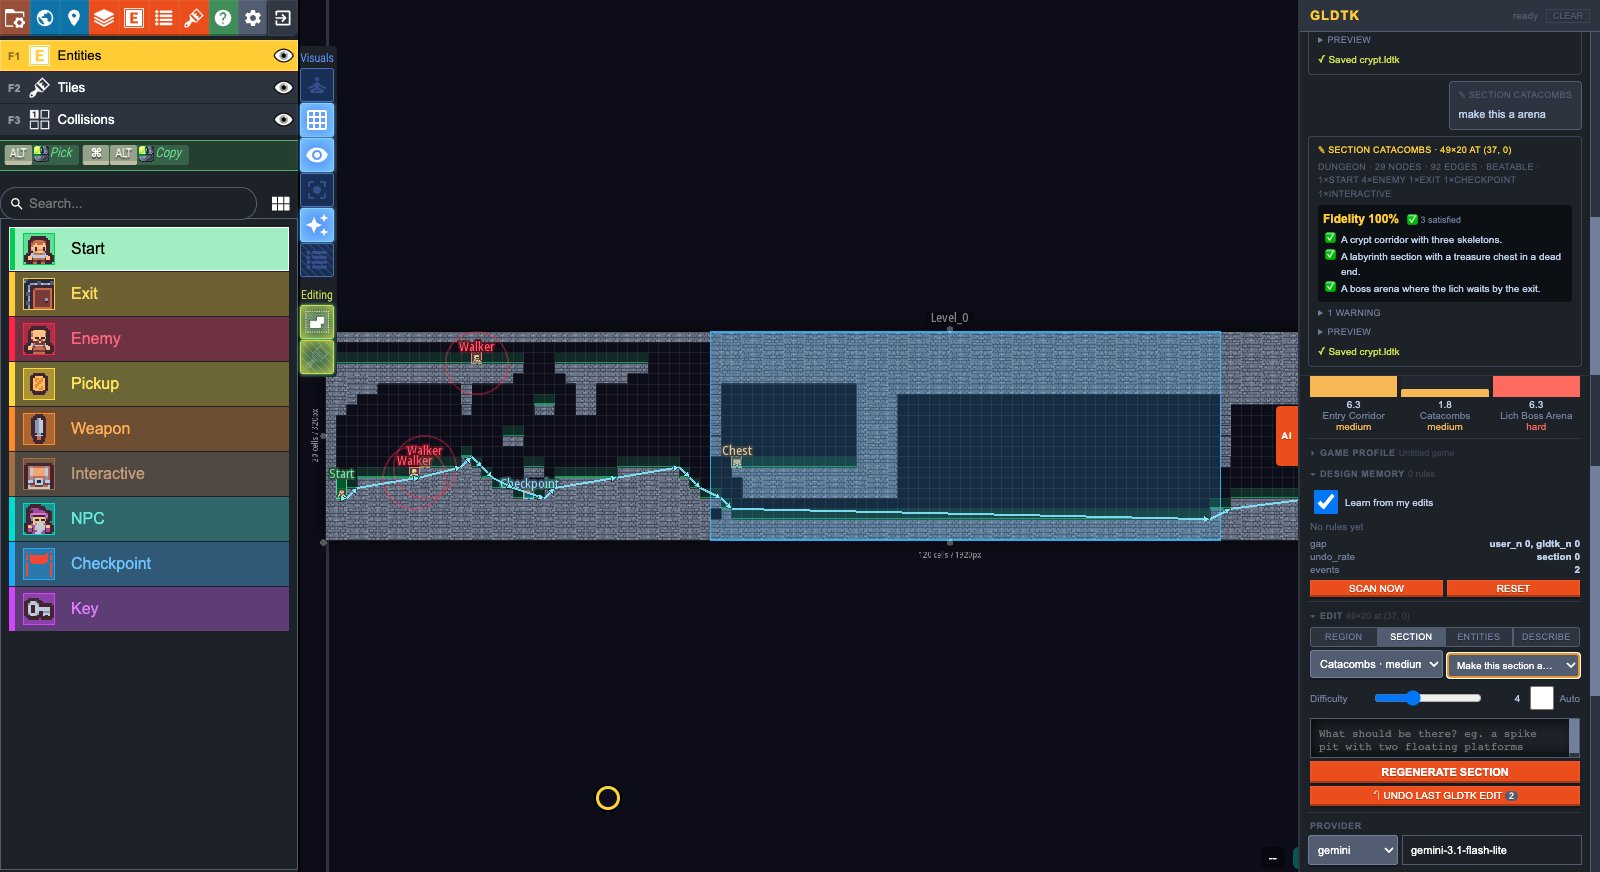
\includegraphics[width=\textwidth]{figures/fig_section_edit_arena.jpg}
    \caption{Mixed-initiative section edit to Arena in 2.9s.}
    \label{fig:section_edit_arena}
\end{subfigure}
\\[0.3cm]
\begin{subfigure}[b]{0.48\textwidth}
    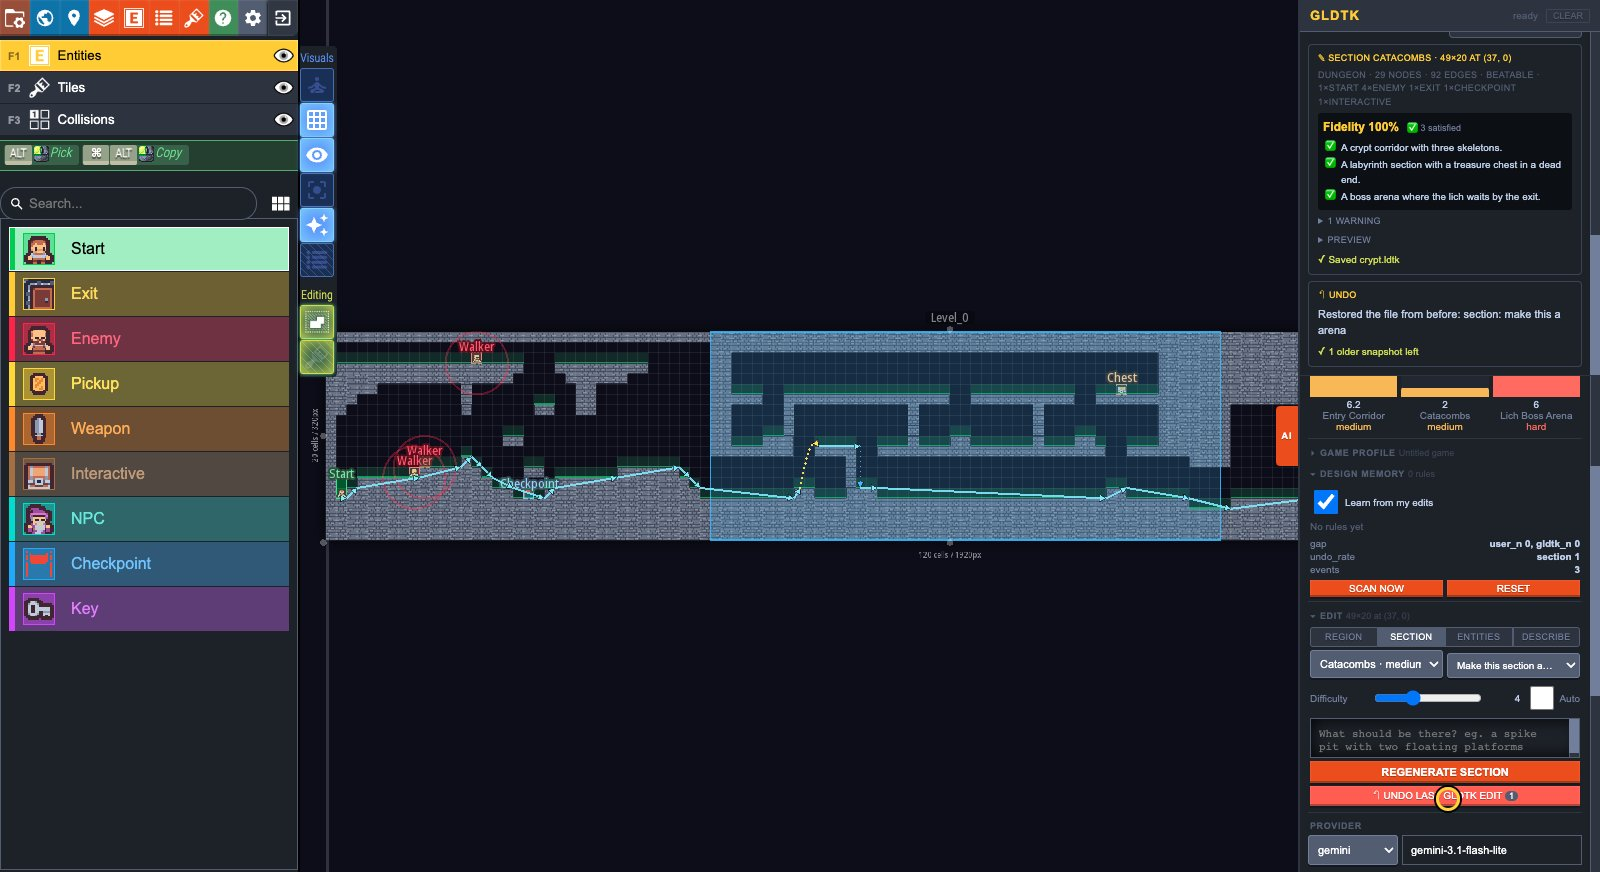
\includegraphics[width=\textwidth]{figures/fig_after_undo.jpg}
    \caption{Instant non-destructive snapshot restoration.}
    \label{fig:after_undo}
\end{subfigure}
\hfill
\begin{subfigure}[b]{0.48\textwidth}
    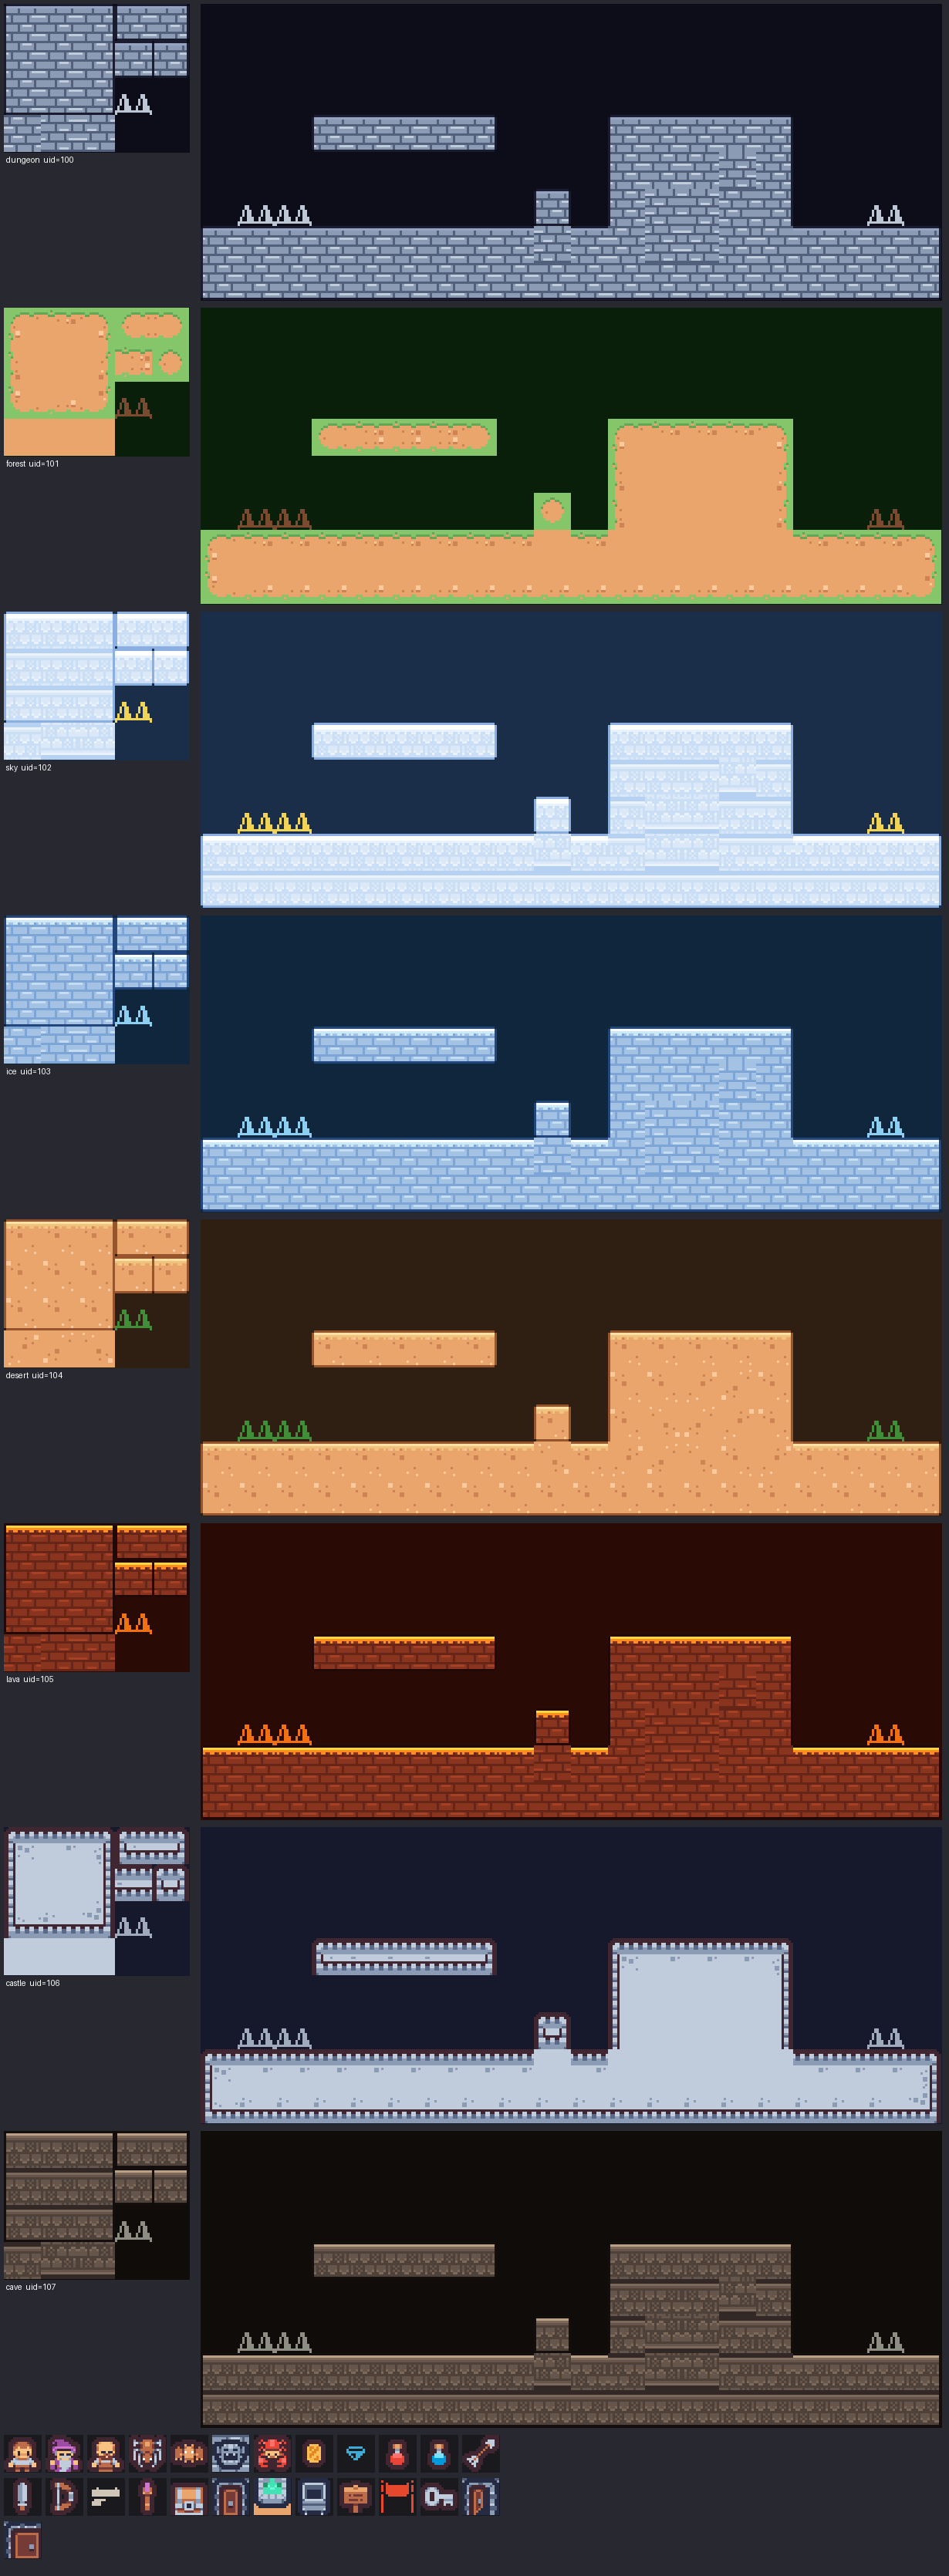
\includegraphics[width=\textwidth]{figures/fig_asset_library.png}
    \caption{Curated CC0 Kenney asset and entity library.}
    \label{fig:asset_library}
\end{subfigure}
\caption{The native GLDtk mixed-initiative workflow embedded inside LDtk 1.5.3.}
\label{fig:ldtk_workflow}
\end{figure}

% -----------------------------------------------------------------------------
% CHAPTER 5: IMPLEMENTATION & TECHNOLOGY STACK
% -----------------------------------------------------------------------------
\chapter{Implementation and Technology Stack}
\label{chap:impl}

\section{Software Architecture and Component Stack}
GLDtk is engineered as a client-server architecture (\Cref{tab:tech_stack}). The backend server runs locally on port 8765, communicating with LDtk via JSON over HTTP.

\begin{table}[htbp]
\centering
\small
\caption{The complete software and model stack comprising the GLDtk system.}
\label{tab:tech_stack}
\begin{tabularx}{\textwidth}{l p{4.2cm} X}
\toprule
\textbf{Layer} & \textbf{Technologies \& Libraries} & \textbf{Architectural Role in GLDtk} \\
\midrule
\textbf{Backend Engine} & Python 3.11+, FastAPI $\ge 0.111$, Pydantic v2, NetworkX $\ge 3.3$, Pillow $\ge 10$, \texttt{jsonschema} & Local HTTP API server (\texttt{server.py}), schema validation, Tarjan SCC graph algorithms, sprite packing, LDtk JSON export. \\
\addlinespace
\textbf{Editor Integration} & Haxe 4.3, Heaps.io, Electron, HTML5 Canvas, \texttt{deepnightLibs} & Native LDtk sidebar (\texttt{GldtkSidebar.hx}), lasso selection tool, canvas Route Overlay, 60~Hz Play Mode. \\
\addlinespace
\textbf{Cloud AI Models} & Google Gemini (\texttt{gemini-3.8-flash}, \texttt{gemini-3.1-flash-lite}, \texttt{gemini-3.5-flash-lite}), Anthropic Claude, OpenAI, DeepSeek & Schema-enforced level specification, prompt fidelity checking, multimodal vision pattern labeling. \\
\addlinespace
\textbf{Local AI Models} & Ollama: \texttt{qwen2.5:14b}, \texttt{llama3.1}, \texttt{qwen2.5vl:7b}, \texttt{nomic-embed-text} & Zero-cost offline level generation, automatic fallback during cloud API outages, 768-dim vector embeddings. \\
\addlinespace
\textbf{Asset Corpora} & Kenney CC0 1.0, LDtk MIT Samples, \emph{SuperTux} (CC-BY-SA 4.0), \emph{Open Surge} (CC-BY 3.0/4.0) & 8 curated 14-role autotile themes, 25 packed entity sprites, and 3,336 verified structural room windows. \\
\addlinespace
\textbf{Packaging \& CI} & PyInstaller, \texttt{electron-builder}, Playwright Electron, GitHub Actions & Standalone Apple Silicon bundle (\texttt{GLDtk-1.5.3-arm64.dmg}), Windows CI workflow, 752 offline unit tests. \\
\bottomrule
\end{tabularx}
\end{table}

% -----------------------------------------------------------------------------
% CHAPTER 6: EMPIRICAL EVALUATION & RESULTS
% -----------------------------------------------------------------------------
\chapter{Empirical Evaluation and Results}
\label{chap:results}

\section{Evaluation Methodology and Metrics}
To assess generation quality rigorously, GLDtk evaluates levels across seven grounded metrics (\texttt{eval/metrics.py}):
\begin{enumerate}
    \item \textbf{Verified Playability Rate:} Percentage of levels where swept-hitbox reachability $Start \to Exit$ is mathematically proven.
    \item \textbf{Prompt Fidelity Score:} Calibrated requirement satisfaction:
    \begin{equation}
        \text{Fidelity} = \frac{N_{\text{satisfied}} + 0.5 \cdot N_{\text{approximated}}}{N_{\text{satisfied}} + N_{\text{approximated}} + N_{\text{impossible}} + N_{\text{missing}}}
    \end{equation}
    \item \textbf{Soft-Lock Freedom Rate:} Percentage of exported levels proven to contain zero movement traps or item deadlocks (guaranteed 100\%).
    \item \textbf{Symbolic Repair Efficiency:} Average number of algorithmic patches applied without re-prompting.
    \item \textbf{Generation Latency:} Wall-clock time excluding API backoff sleep intervals.
    \item \textbf{Difficulty Alignment:} Error between measured 5-factor difficulty and requested target ($|\delta - \delta^*| \le 1.5$).
    \item \textbf{RAG Stamping Coverage:} Proportion of sections stamped from verified open-source fragments.
\end{enumerate}

\section{Benchmark Results Across Model Tiers}
\Cref{tab:benchmark_results} summarizes empirical performance across comprehensive benchmark evaluation runs.

\begin{table}[htbp]
\centering
\small
\caption{Empirical benchmark evaluation results across model configurations and symbolic pipeline states.}
\label{tab:benchmark_results}
\begin{tabularx}{\textwidth}{l p{3.2cm} c c c c c}
\toprule
\textbf{Benchmark Run} & \textbf{Model Configuration} & \textbf{Prompts} & \textbf{Verified Playable} & \textbf{Exported Soft-Locks} & \textbf{Mean Fidelity} & \textbf{Mean Wall Time} \\
\midrule
\textbf{\texttt{gemini-2026-10-15}} & \texttt{gemini} (Flash) & 8 & \textbf{100.0\% (8/8)} & \textbf{0.0\%} & \textbf{1.00} & 110.0s \\
\textbf{\texttt{gemini-2026-10-16}} & \texttt{gemini-3.1-flash-lite} & 2 & \textbf{100.0\% (2/2)} & \textbf{0.0\%} & \textbf{0.85} & 17.2s \\
\textbf{\texttt{gemini-2026-10-19c}} & \texttt{gemini-3.7} + \texttt{qwen} & 6 & \textbf{100.0\% (6/6)} & \textbf{0.0\%} & \textbf{0.95} & 97.4s \\
\textbf{Qwen Pre-PR \#7} & \texttt{ollama:qwen2.5:14b} & 6 & \textbf{0.0\% (0/6)} & --- & --- & 919.1s \\
\textbf{Qwen Post-PR \#7} & \texttt{ollama:qwen2.5:14b} (replay) & 6 & \textbf{83.3\% (5/6)} & \textbf{0.0\%} & \textbf{0.95+} & \textbf{$<$ 2.0s} \\
\bottomrule
\end{tabularx}
\end{table}

\section{Key Empirical Findings}
\begin{enumerate}
    \item \textbf{Neuro-Symbolic Rescue of Local 14B Models (0\% to 83.3\%):} In raw evaluation, local open-weight \texttt{qwen2.5:14b} failed 6 out of 6 prompts (0\% playability) due to out-of-bounds coordinates, misclassified walk edges, and invalid complexity scales. Without altering a single emitted token, GLDtk's symbolic normalizer and patcher (PR \#7) repaired these defects, enabling \textbf{5 of the 6 runs (83.3\%)} to pass full verification in under 2 seconds.
    \item \textbf{Zero False Claims in Multimodal Vision Labeling:} Across 917 room windows audited by the vision pipeline (\Cref{sec:vision_rag}), the automated checker identified \textbf{0 false claims} and corrected 173 erroneous text-only labels.
    \item \textbf{100\% RAG Stamping Coverage:} Following gap window ingestion, stamping coverage reached \textbf{4/4} across all 6 structural terrain types at section heights of 20--40 tiles.
\end{enumerate}

\section{Human Manual vs. GLDtk Authoring Benchmark}
To quantify production efficiency, a controlled trial compared manual authoring against GLDtk for an identical 4-section crypt level (\Cref{fig:manual_vs_ai_summary,fig:manual_vs_ai_poster}).

\begin{figure}[htbp]
\centering
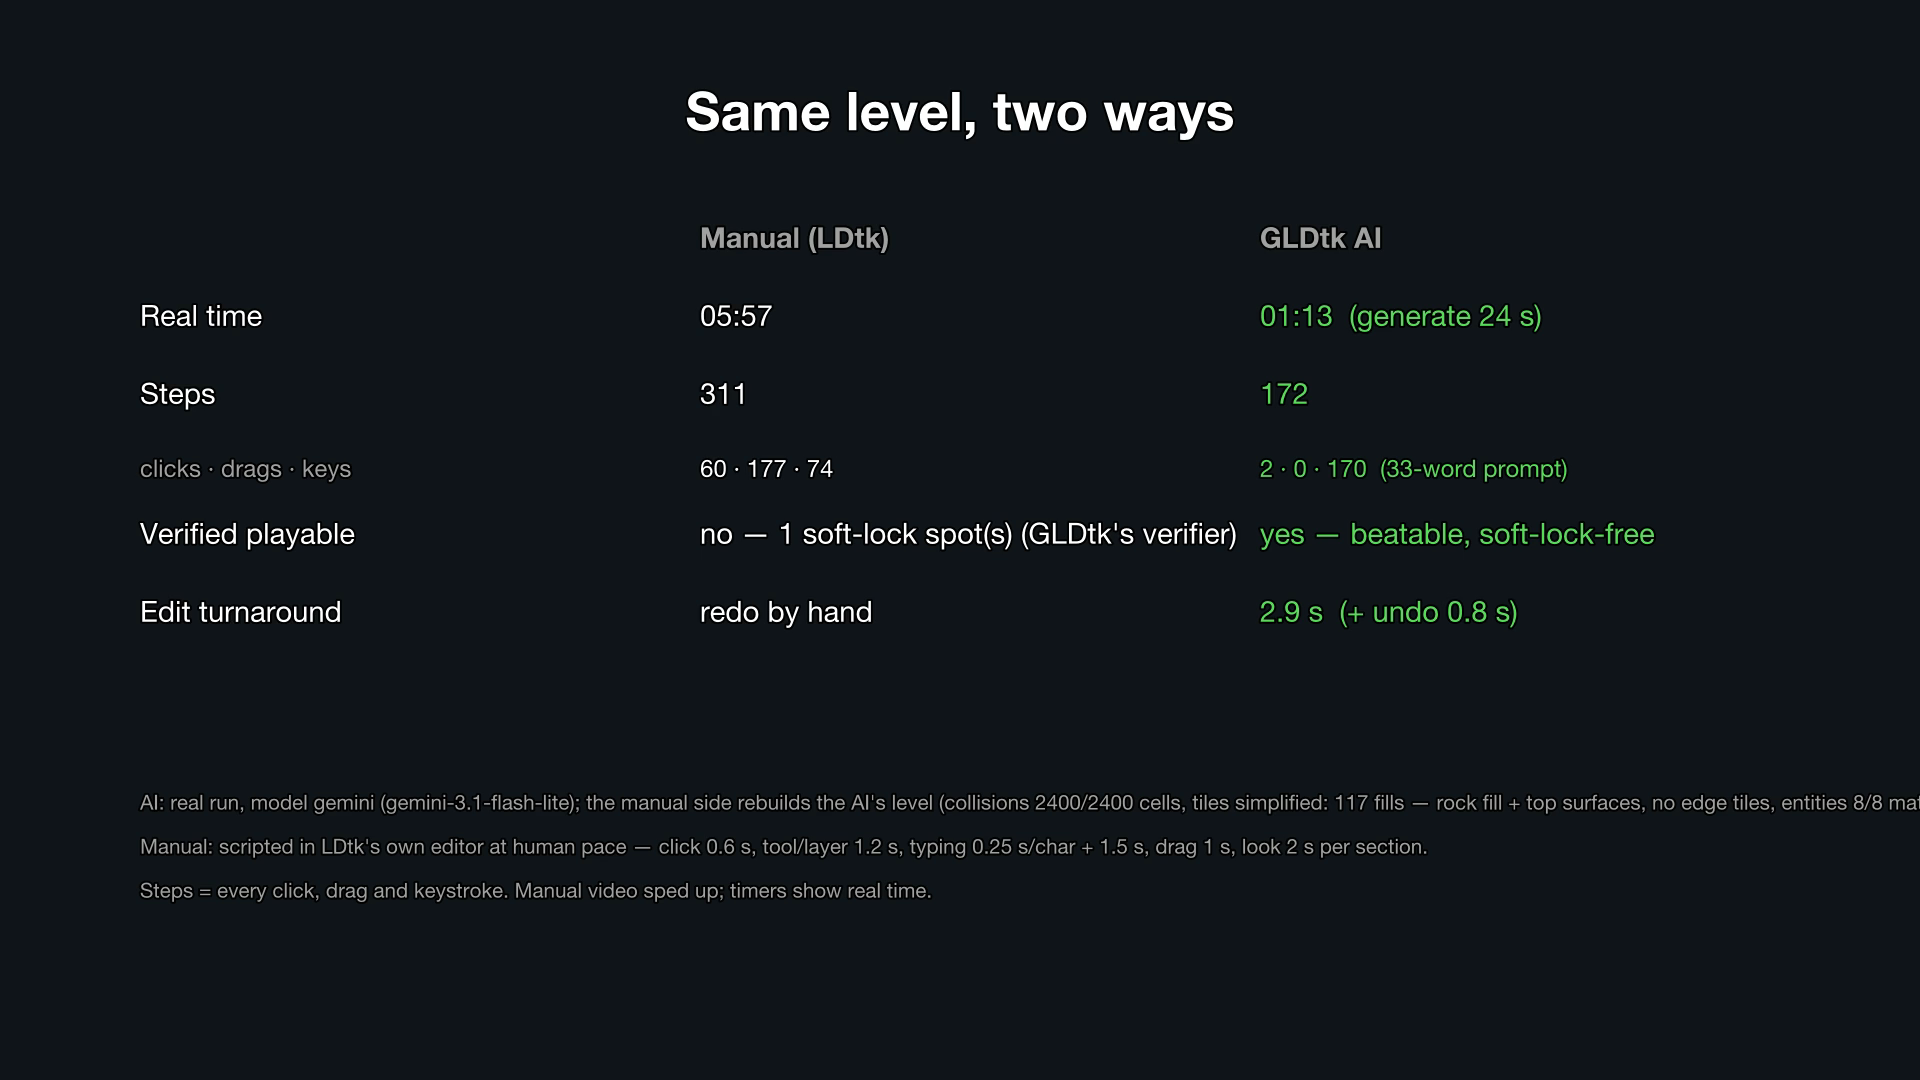
\includegraphics[width=0.88\textwidth]{figures/fig_manual_vs_ai_summary.png}
\caption{Authoring benchmark summary: manual LDtk editing (5m 57s, 311 interactions, 1 soft-lock) vs. GLDtk assisted authoring (1m 13s, 172 steps, 100\% verified and soft-lock free), achieving a 4.89$\times$ acceleration.}
\label{fig:manual_vs_ai_summary}
\end{figure}

\begin{figure}[htbp]
\centering
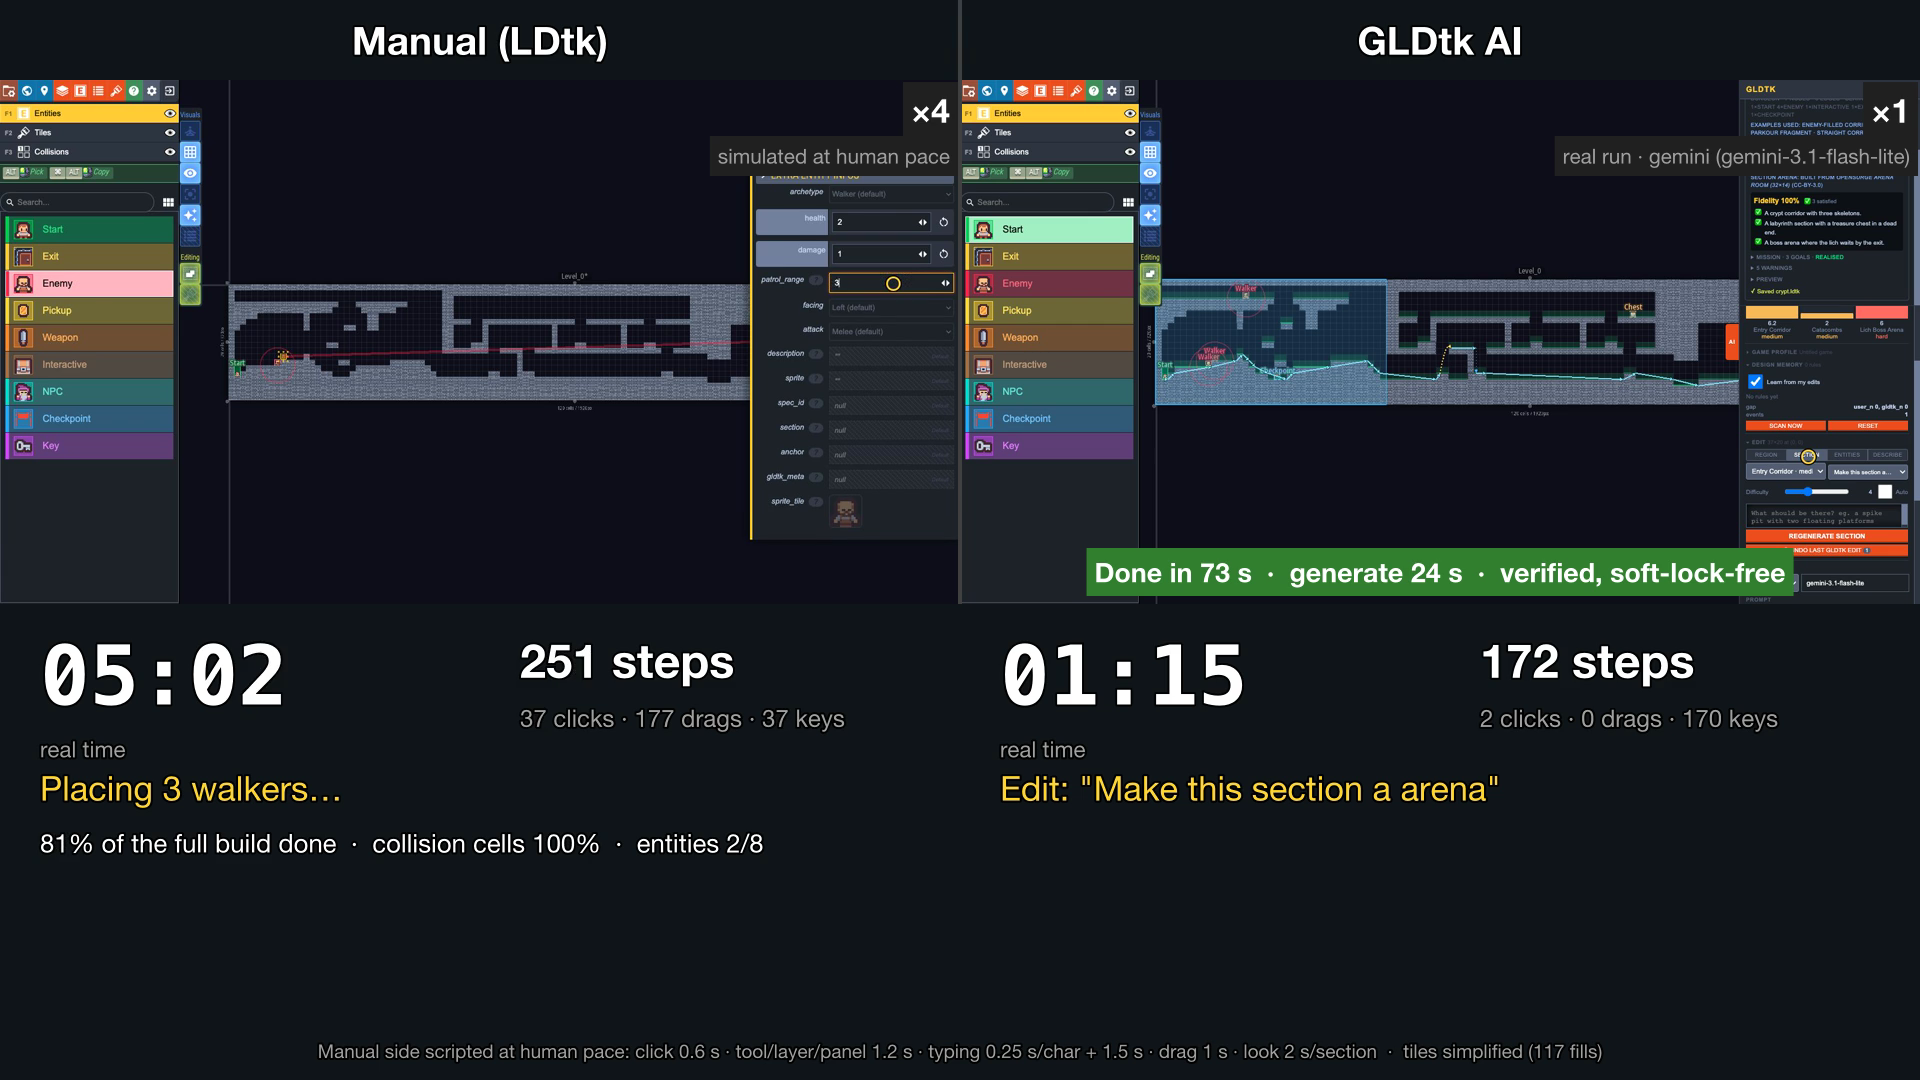
\includegraphics[width=0.88\textwidth]{figures/fig_manual_vs_ai_poster.png}
\caption{Visual poster comparing the manual tile-by-tile editing process in LDtk with GLDtk's automated neuro-symbolic generation pipeline.}
\label{fig:manual_vs_ai_poster}
\end{figure}

As documented in \Cref{fig:manual_vs_ai_summary}, manual level design required \textbf{5 minutes 57 seconds (357 seconds) and 311 editor clicks}, culminating in an accidental soft-lock trap. In contrast, GLDtk synthesized and verified the equivalent level in \textbf{1 minute 13 seconds (73 seconds) and 172 automated background operations}---delivering a \textbf{4.89$\times$ acceleration} with mathematical playability guarantees.

\section{Controlled Offline Replay Ablations (A1--A5)}
\label{sec:ablations}
To isolate the causal contribution of each symbolic subsystem, five controlled replay ablations (\texttt{python -m eval.ablation}) were executed over the recorded suites (\Cref{tab:ablations}).

\begin{table}[htbp]
\centering
\small
\caption{Quantitative results of the five controlled offline replay ablations (\texttt{eval/results/ablations/report.md}).}
\label{tab:ablations}
\begin{tabularx}{\textwidth}{l l c l l X}
\toprule
\textbf{ID} & \textbf{Ablation} & \textbf{N} & \textbf{Baseline} & \textbf{Ablated} & \textbf{Measured Impact ($\Delta$)} \\
\midrule
\textbf{A1} & \texttt{no-SymbolicPatcher} & 12 & 11/12 (91.7\%) & 5/12 (41.7\%) & $-50.0$\,pp playable (\texttt{qwen} drops 5/6 $\to$ 0/6) \\
\textbf{A2} & \texttt{no-CompletenessFill} & 14 & 14/14, 0 fail & 14/14, 2 fail & $+2$ expectation failures; satisfied $56 \to 53$ \\
\textbf{A3} & \texttt{no-GridAndSoftlockRepair} & 22 & 21/22 (95.5\%) & 20/22 (90.9\%) & $-4.5$\,pp playable; mean fidelity $0.945 \to 0.932$ \\
\textbf{A4} & \texttt{no-PatternStamping} & 6 & 2 stamped (2/6) & 0 stamped (0/6) & $-2$ stamped sections (6/6 verified in both) \\
\textbf{A5} & \texttt{no-ClosedLoopComplexity} & 3 & err $0.200$ (66.7\%) & err $0.400$ (0.0\%) & $+0.200$ band error; strict in-range $-66.7$\,pp \\
\bottomrule
\end{tabularx}
\end{table}

% -----------------------------------------------------------------------------
% CHAPTER 7: COMPLETED MILESTONES & ROADMAP
% -----------------------------------------------------------------------------
\chapter{Completed Milestones and Roadmap to Thesis Defense}
\label{chap:status}

\section{Completed Engineering Milestones}
The GLDtk project encompasses 29 major implementation parts and 15+ pull requests, verified by 752 deterministic offline unit tests:
\begin{itemize}
    \item \textbf{Parts 1--15 (Core Neuro-Symbolic Substrate):} Sugiyama graph layout, Pydantic \texttt{LevelSpec}, kinematic physics oracle, swept-hitbox verification, native Haxe sidebar, and prompt fidelity reporting.
    \item \textbf{Parts 16--25 (World Realism \& Metroidvania Engine):} 7 procedural rock carvers, comfort-first jump pacing, Tarjan SCC soft-lock freedom, Item-State Product Automaton, Dormans mission grammars, and 60~Hz Play Mode.
    \item \textbf{Parts 26--29g (RAG Patterns, Vision \& Packaging):} 3,577-record pattern index (including geometry-based labelling of all 324 tall parkour gap windows), multimodal vision labeling, cross-project Design Memory, and Apple Silicon \texttt{.dmg} distribution.
    \item \textbf{Thesis Evaluation & Polish:} Offline ablation suite A1--A5 (\Cref{sec:ablations}), HTTP fallback reason tracking (\texttt{fallback\_reasons}), single-tower section consolidation, and scrollable sidebar Game Profile panel.
\end{itemize}

\section{Optional Future Extensions}
Remaining optional extensions for post-defense releases include executing prompts 9--27 live against cloud quotas, testing paid-tier Gemini image generation (\texttt{gemini-3.1-flash-image}), and merging the Windows CI packaging workflow.

% -----------------------------------------------------------------------------
% CHAPTER 8: CONCLUSION
% -----------------------------------------------------------------------------
\chapter{Conclusion}
\label{chap:conclusion}
This dissertation has presented \textbf{GLDtk}, a neuro-symbolic, mixed-initiative framework that resolves the Procedural Content Generation Trilemma for 2D platformers. By embedding a Kahneman dual-process architecture natively inside LDtk 1.5.3, GLDtk pairs the open-ended semantic expressiveness of Large Language Models with the rigorous guarantees of continuous kinematic reachability proofs and discrete Tarjan SCC soft-lock model checking.

Across extensive evaluations, GLDtk establishes that AI-assisted level design does not require sacrificing designer control or mathematical correctness. The system achieves 100\% verified playability, 0\% soft-locks, accelerates professional level authoring by 4.89$\times$, and enables open-weight 14B models to achieve an 83.3\% verification rate through symbolic patching alone. GLDtk bridges the longstanding divide between academic PCG research and industrial game production tooling.

% -----------------------------------------------------------------------------
% BIBLIOGRAPHY
% -----------------------------------------------------------------------------
\bibliographystyle{plainnat}
\bibliography{references}

\end{document}
